\part{Radiative Transfer}\label{Radiative Transfer}

\section*{Introduction}

This section of the course was lectured by \href{https://users.physics.ox.ac.uk/~pierrehumbert/}{Raymond T. Pierrehumbert} covering basic atmospheric Radiative Transfer. In the academic year 2024-2025, Ray did not cover scattering, so I will not cover scattering in these notes.\vspace{5 mm}

\noindent This section consists of four chapters:\vspace{5 mm}

\begin{enumerate}
    \item \hyperref[Basic Thermodynamics]{Basic Radiation Concepts}: 
        
        \begin{quote}
            We introduce the basic vocabulary needed to describe radiative transfer. We first characterise the radiation field, including how to encode the \hyperref[Solid Angle Box]{direction} and \hyperref[Radiance Box]{magnitude} of radiation. Next, we describe how objects emit and absorb radiation.
        \end{quote}

    \item Molecular Spectroscopy: 
    
        \begin{quote}
            We detail how we characterise \hyperref[Line Box]{spectral lines} in terms of certain parameters. We then discuss how those parameters are determined physically, and introduce some explicit functional forms such as the \hyperref[Lorentz Box]{Lorentz Line Shape}.
        \end{quote}
    
    \item Schwarzschild Equation:
        
        \begin{quote}
            We formulate an equation for radiative transfer throughout the atmosphere and solve it. We  
        \end{quote}
    \item Radiative Equilibrium:
        
        \begin{quote}
            We make the grey gas approximation in order to analyse how an atmosphere would behave in pure radiative equilibrium: i.e., if radiation were the dominant energy transport mechanism.
        \end{quote}
\end{enumerate}

\chapter{Basic Radiation Concepts}

\section{Direction of Radiation: Rays and Solid Angle}

In general, radiation will not only be a function of position $\vec{r}$ but will also be a function of direction\footnote{This is why your eyes will hurt if you look directly at the sun but they won't if you look at these lecture notes.}. We can encode the direction in which radiation is propagating with a \textbf{ray}, a vector $\vec{\omega}$ of (dimensionless) length $1$ on a unit sphere. $\vec{\omega}$ encodes information regarding the direction of propagation, but not regarding the magnitude (e.g., energy) of the radiation. In Cartesian coordinates, this is:
\begin{align}
    \vec{\omega}=\left(\begin{array}{ccc}
         \sin(\theta)\cos(\phi)\\
         \sin(\theta)\sin(\phi)\\
         \cos(\theta)
    \end{array}\right)
\end{align}

We also define the \textbf{Solid Angle}, which is a measure of a set of rays, with units of \textbf{Steradians} (\qty{}{\steradian}). In other words, \textbf{solid angle} encodes from \textit{how many} directions some radiation is coming from. For example, if radiation is propagating towards you from every direction, the \textbf{solid angle} of that will be larger than if radiation were only propagating towards you from a single direction.

We can make this more intuitive by drawing an analogy between the solid angle in 3D (measured in \textbf{steradians} (\qty{}{\steradian})) and the angle in 2D angle (measured in radians (\qty{}{\radian})). In 2D, radians measure an angle by relating the circumference of a circle to the arc length subtended by that angle (see Fig. \ref{2D Ray}). For example, $1\pi$ \qty{}{\radian} corresponds to an angle that subtends half a unit circle ($180$ degrees) and thus an arc length of $1\pi$. Analogously, steradians measure a solid angle by relating the surface area of a sphere to the patch subtended by a solid angle (see Fig. \ref{3D Ray}). For example, a set of rays pointing in all directions has a solid angle of $4\pi$ \qty{}{\steradian}, while a set of rays with some positive $x$ component (i.e., $\sin(\theta)\cos(\phi)>0$) has a solid angle of $2\pi$ \qty{}{\steradian}.

Often we will have to integrate over solid angles/directions (as radiation will be a continuous function of $\vec{\omega}$) in the same way that we might integrate over angles. We therefore introduce the differential solid angle:

\begin{fact}{Solid Angle}{Solid Angle Box}\label{Solid Angle Box}
    The solid angle $\Omega$ is a dimensionless area encoding how many directions we are considering, and is measured in steradians \qty{}{\steradian}. We define the differential solid angle $d\Omega$:
    \begin{gather}
        \BOX{d\Omega=d\theta \sin\theta \,d\phi}\\
        \BOX{\Omega = \iint\displaylimits_\text{directions considered} d\Omega}
    \end{gather}
    \begin{figure}[H]
        \centering
        \begin{subfigure}{0.4\linewidth}
            \centering
            \scalebox{1.4}{
            \begin{tikzpicture},
                \draw[->] (0,0) -- (1.5,0) node[anchor=west] {$x$};
                \draw[->] (0,0) -- (0,1.5) node[anchor=south] {$y$};
                \draw[dashed] (0,0) circle [radius=1.5cm];
                %\draw (3mm,0mm) arc [start angle=0, end angle=225, radius=3mm];
                \coordinate (A) at (0,0);
                \coordinate (B) at (225:1.5cm);
                \coordinate (C) at (1.5,0);
                \coordinate (D) at (240:1.5cm);
                \draw (C) -- (A) -- (B)
                    pic [draw=black, fill=myorange,angle radius=4mm, opacity=0.5] {angle = C--A--B};
                \draw (B) -- (A) -- (D)
                    pic [draw=mydarkblue, angle radius=15mm] {angle = B--A--D};
                \draw[->,ultra thick] (0,0) -> (225:1.5cm) node[anchor=south] {$\vec{\omega}$};
                \node at (-1.2,-1.4) {$d\theta$};
                \node at (-0.15,0.15) {$\theta$};
                \draw[->] (0,0) -> (240:1.5cm) ;%node[anchor= west] {$\vec{\omega}+\vec{d\omega}$};
            \end{tikzpicture}}
            \caption{2D Ray ($\vec{\omega}$), Angle ($\theta$), and Differential Angle ($d\theta$)}
            \label{2D Ray}
        \end{subfigure}
        \qquad
        \begin{subfigure}{0.4\linewidth}
            \centering
            \scalebox{1.4}{
            \begin{tikzpicture},
                \begin{scope}[3d view={135}{25.26}]
                    \draw[->] (0,0,0) -- (1.5,0,0) node[anchor=north west] {$x$};
                    \draw[->] (0,0,0) -- (0,1.5,0) node[anchor=north] {$y$};
                    \draw[->] (0,0,0) -- (0,0,1.5) node[anchor=north west] {$z$};
                    \draw[-,dashed] plot[domain=0:400,samples=41,smooth]({1.5*sin(\x)},{1.5*cos(\x)},{0});
                    \draw[-,dashed] plot[domain=0:400,samples=41,smooth]({1.5*cos(0)*sin(\x)},{1.5*sin(0)*sin(\x)},{1.5*cos(\x)});
                    \coordinate (A) at (-0.294,0.808,1.228);
                    \coordinate (B) at (-0.294,0.808,0);
                    \filldraw[fill=myorange,opacity=0.5] (0,0,0.732) .. controls +(-0.015,0.04,0) and +(0,0,0.1) .. (-0.137,0.394,0.604) -- (0,0,0);
                    \draw[->,ultra thick] (0,0,0) -> (A) node[anchor=west] {$d\Omega$};
                    \draw[dotted] (A) -- (B) -- (0,0,0);
                    \filldraw[fill=mydarkblue,opacity=0.8] (A) circle [radius=0.1cm];
                    \filldraw[fill=myorange,opacity=0.5] (0.840,0,0) .. controls +(0,0.8,0) and +(0.5,0.2,0) .. (B) -- (0,0,0);
                \end{scope}
                \begin{scope}
                    \draw[-,dashed] plot[domain=0:400,samples=41,smooth]({1.5*sin(\x)},{1.5*cos(\x)});
                    \node at (0.15,0.4) {$\theta$};
                    \node at (0,-0.2) {$\phi$};
                    \node at (0.5,0.3) {$\vec{\omega}$};
                \end{scope}
            \end{tikzpicture}}
            \caption{3D Ray ($\vec{\omega}$), Angle ($\theta,\phi$),and Differential Solid Angle ($d\Omega$)}
            \label{3D Ray}
        \end{subfigure}
        \caption{Rays, Angles, and Differential Solid Angle}
    \end{figure}
\end{fact}
One can integrate this differential over the entire sphere ($\theta\in[0,\pi],\phi\in[0,2\pi]$) to readily verify that the solid angle over an entire sphere is $4\pi$ \qty{}{\steradian}, and over half a sphere ($\theta\in[0,\pi/2],\phi\in[0,2\pi]$) is $2\pi$ \qty{}{\steradian}. Intuitively, the differential solid angle is the dimensionless area element in spherical coordinates. Think of the small rectangle with side lengths $r\,d\theta$ and $r\sin\theta \,d\phi$, but you divide by $r^2$ to make it dimensionless. This is analogous to the case in 2D, where the differential angle is a dimensionless line element in radial coordinates. Think, analogously, of a small line of side length $r\,d\theta$, but again you divide by $r$ to make it dimensionless.

We also define the \textbf{projected} differential solid angle. This accounts for the fact that if we have some surface which is absorbing radiation, radiation parallel to the surface will not be absorbed.
\begin{align}
    \BOX{d\Omega_\perp=\cos\zeta\,d\Omega}
\end{align}
where $\zeta$ is the \textbf{zenith angle}, the angle between the ray ($\vec{\omega}$) and the ray normal to the surface in question. Sometimes we orient our axes such that $\theta=\zeta$ because it simplifies the system, but note that we do not always do this nor does this always simplify the situation.

\section{Magnitude of Radiation: (Spectral) Radiance and (Spectral) Irradiance}

Now that we have learnt how to characterise the \textit{direction} in which radiation if propogating, we wish to characterise the \textit{magnitude} of the radiation. 

Let us consider some surface \textit{perpendicular} to some radiation propogating through it. The \textbf{Radiance} $I$ is the energy flux of the radiation flowing through that surface per unit \textit{time} per unit \textit{area} per unit \textit{solid angle}. $I$ has units of \qty{}{\joule\per\second\per\metre\squared\per\steradian}. Now consider an \textit{arbitrarily} oriented surface, which is oriented with at some \textbf{zenith angle} $\zeta$ to some radiation. Then the energy flux $\phi$ (in units of \qty{}{\joule\per\second}) is calculated by integrating the \textbf{radiance} over solid angles and the area of the patch as follows:
\begin{align}
\phi=\iint\,I\,d\Omega_\perp\,dA
\end{align}

The \textbf{Irradiance} $E$ is the energy flux flowing perpendicular through that surface per unit time and unit area. E has units of \qty{}{\joule\per\second\per\metre\squared}. The two are related as follows:
\begin{gather*}
    E=\int_{\Omega_\pm} I\,d\Omega_\perp \\
    \phi=\int E\,dA
\end{gather*}

Often times radiation is only propagating from one hemisphere (i.e., from one direction) so we integrate over the upwards or downwards propagating hemisphere, which we denote as $\Omega_+$ and $\Omega_-$, respectively. I also remind you that $E$ cannot be a function of $\vec{\omega}$ but $I$ generally is.

So far our discussion has been completely general, but now we focus on light/electromagnetic radiation, which is a wave and thus has a frequency/wavelength. The \textbf{Spectral Radiance} $L$ and \textbf{Spectral Irradiance} $F$ is the radiance and irradiance (respectively) at a given frequency per unit frequency. $L$ and $F$ have units of \qty{}{\joule\per\second\per\metre\squared\per\steradian\per\hertz} and \qty{}{\joule\per\second\per\metre\squared\per\hertz}, respectively. Equivalently, $L(\nu)\,d\nu$ is the radiance carried by waves with some frequency $\nu'\in[\nu,\nu+d\nu]$ and $F(\nu)\,d\nu$ is the irradiance carried by waves with some frequency $\nu'\in[\nu,\nu+d\nu]$. Due to the laws of electromagnetism, the total energy of a superposition of electromagnetic waves is given by the sum of the energy of the waves at each frequency. As such:
\begin{align}
    I&=\int L\,d\nu\\
    E&=\int F\, d\nu\\
    \phi&=\iint\,L\,d\nu\,d\Omega_\perp\,dA
\end{align}

Since the spectral radiance at any point is typically a function of both $\nu$ and $\vec{\omega}$, we must integrate over both $\nu$ and $\vec{\omega}$ to obtain the radiative energy fluxes per unit area. Practically, this integration cannot be solved analytically and so is done numerically. In these notes, we will make a few approximations in order to make analytical progress/extract physical intuition. We will approximate the distribution over $\vec{\omega}$ (the \textit{Two-Stream Approximation} in \ref{Two Stream Approximation}), integrate over frequency bands (\ref{Frequency Bands}), and make the (bad) grey gas approximation ($\frac{\partial L}{\partial \nu}=0$) in Section \ref{Radiative Equilibrium}.

As a summary:
\begin{fact}{Characterising the Magnitude of Radiation}{Radiance Box}\label{Radiance Box}
    Consider some radiation propagating through a surface at some \textbf{zenith angle} $\zeta$ (i.e., the radiation is at angle $\zeta$ to the vector normal to the surface). Let the power flux in \qty{}{\joule\per\second} through the surface be $\phi$ and the area $A$. Then we define:\vspace{3 mm}

    \begin{minipage}{.5\linewidth}
        \begin{tcolorbox}[colback=myyellow!50!white,colframe=mymagenta]
            \textbf{Radiance} $I$: The energy flux per unit time, area, and solid angle parallel to the direction the radiation is propogating in.
            \begin{align*}
                I&=\frac{\partial^2 \phi}{\partial A \, \partial \left( \Omega \cos\zeta  \right)}\\
                &=\frac{\text{Power flux \textbf{parallel} to \textbf{radiation}}}{\text{per }(\text{Area})(\text{Solid Angle})}
            \end{align*}
        \end{tcolorbox}
        \begin{tcolorbox}[colback=myyellow!50!white,colframe=mymagenta]
            \textbf{Spectral Radiance} $L$: The energy flux per unit time, area, solid angle, and frequency parallel to the direction the radiation is propogating in.
            \begin{align*}
                L&=\frac{\partial^3 \phi}{\partial A \, \partial \left( \Omega \cos\zeta  \right)\,\partial \nu}\\
                &=\frac{\text{Power flux \textbf{parallel} to \textbf{radiation}}}{\text{per }(\text{Area})(\text{Solid Angle})(\text{Frequency})}
            \end{align*}
        \end{tcolorbox}
    \end{minipage}
    \begin{minipage}{.5\linewidth}
        \begin{tcolorbox}[colback=myyellow!50!white,colframe=mymagenta]
            \textbf{Irradiance} $E$: The energy flux per unit time and area through the surface in question.
            \begin{align*}
                F&=\frac{\partial \phi}{\partial A}
                \\&
                =\frac{\text{Power flux \textbf{through} the \textbf{surface}}}{\text{per }(\text{Area})}
            \end{align*}
        \end{tcolorbox}
        \begin{tcolorbox}[colback=myyellow!50!white,colframe=mymagenta]
            \textbf{Spectral Irradiance} $F$: The energy flux per unit time, area, solid angle, and frequency through the surface in question.
            \begin{align*}
                F&=\frac{\partial^2 \phi}{\partial A \, \partial\nu}\\
                &=\frac{\text{Power flux \textbf{through} the \textbf{surface}}}{\text{per }(\text{Area})(\text{Frequency})}
            \end{align*}
        \end{tcolorbox}
    \end{minipage}

    \begin{tikzpicture}
        \node[] at (0,0) {Spectral Radiance: $L$};
        \node[] at (12,0) {Spectral Irradiance: $F$};
        \node[] at (0,-3) {Radiance: $I$};
        \node[] at (12,-3) {Irradiance: $E$};
        \draw (2.5,0) -- (9.5,0);
        \draw (0,-0.5) -- (0,-2.5);
        \draw (12,-0.5) -- (12,-2.5);
        \draw (2.5,-3) -- (9.5,-3);
        \node[isosceles triangle,draw,fill=black,inner sep=0pt,minimum size =0.2cm] at (6,0){};
        \node[] at (6,0.5) {$\int d\Omega_\perp$};
        \node[isosceles triangle,draw,fill=black,inner sep=0pt,minimum size =0.2cm] at (6,-3){};
        \node[] at (6,-2.5) {$\int d\Omega_\perp$};
        \node[isosceles triangle,draw,rotate=270,fill=black,inner sep=0pt,minimum size =0.2cm] at (0,-1.5){};
        \node[] at (1,-1.5) {$\int d\nu$};
        \node[isosceles triangle,draw,rotate=270,fill=black,inner sep=0pt,minimum size =0.2cm] at (12,-1.5){};
        \node[] at (11,-1.5) {$\int d\nu$};
    \end{tikzpicture}
\end{fact}


\subsection{Frequency, Wavelength, and Wavenumber}

So far, we have specified how quickly a wave oscillates by refering to its frequency $\nu$, but we could have referred to its wavelength $\lambda$ or its wavenumber $\tilde{\nu}$. All of these give you the same information, and you can freely convert between them if you know the speed of the wave $c$. For light, this is $c\approx$ \qty{3e8}{\metre\per\second}. You can find the information summarised in the table below.
\begin{figure}[H]
    \begin{tabular}{|p{1.4cm}|p{2.8cm}|p{1.6cm}|p{9.6cm}|}
        \hline
            Symbol & Name & Units & Meaning \\
        \hline
        \hline
        $\nu$ & Frequency & \qty{}{\per\second} ; \qty{}{\hertz} & The number of oscillations per second.\\
        \hline
        $\lambda$ & Wavelength & \qty{}{\metre} & The peak-to-peak length of the wave. $\nu\lambda=c$\\
        \hline
        $\tilde{\nu}$ & Wavenumber & \qty{}{\per\metre}; \qty{}{\per\centi\metre}  & The wavelengths per unit metre. $\tilde{\nu}=\lambda^{-1}$. In spectroscopy, we often refer to wavenumber in terms of wavelengths per \textit{centimetre} (\qty{}{\per\centi\metre}) for convenient numbers.\\
        \hline
    \end{tabular}
\end{figure}
Finally, we should note two nuances. First, I introduced \textbf{spectral radiance/irradiance} as the radiance/irradiance per unit frequency, but many people refer to the \textbf{spectral radiance/irradiance} as the radiance/irradiance per unit wavelength or per unit wavenumber. The choice of description is ultimately arbitrary, but you should be aware of this potential confusion.

The second nuance is more important. It is the $L(\nu)\,d\nu$ term which is physically meaningful, not the $L(\nu)$ term by itself. This is because, as already mentioned, $\nu$ is only one of the ways we could have chosen represent the property of wavelength/frequency. We could equally use the wavelength $\lambda$. To illustrate the point, let's convert the spectral radiance $L(\nu)\,d\nu$ carried by the radiation with frequency $\nu'\in[\nu,\nu+d\nu]$ to something in terms of the wavelength $\lambda$:
\begin{align*}
    \nu\lambda=c\therefore\,&\\
    L(\nu)\,d\nu=&L\left(\frac{c}{\lambda}\right)\,d\left(\frac{c}{\lambda}\right)\\
    =&\frac{c}{\lambda^2}L\left(\frac{c}{\lambda}\right)\,d\lambda\\
    =&\hat{L}(\lambda)\,d\lambda
\end{align*}

\noindent where we have defined $\hat{L}(\lambda)\equiv\frac{c}{\lambda^2}L\left(\frac{c}{\lambda}\right)$. Notice how the functional form fundamentally changes when we undergo an ultimately arbitrary coordinate transformation from $\nu$ to $\lambda$: the `\textit{frequency} spectral radiance' $L(\nu)$ and `\textit{wavelength} spectral radiance' $L(\lambda)$ are not the identical! But nothing physically \textit{out there} should depend on how we choose to write it down, so we conclude that $L(\nu)$ by itself is an artefact arising from our choice to represent it in terms of $\nu$.

\section{Emission: Black Body Radiation}

Now that can characterise radiation in terms of direction and magnitude, we now aim to lay the foundations of characterising how matter interacts with radiation. We first consider emission here.

A \textbf{black body} is a theoretical object which absorbs all incident electromagnetic radiation. To a good approximation, many stellar bodies are black bodies, including the Sun. One can show that such a body must emit spectral radiance at all times given by $L_{BB}$:
\begin{align}
    \boxed{L_{BB}\,d\nu=B(\nu,T)\,d\nu=\frac{2h\nu^3}{c^2}\frac{1}{\exp\left( \frac{h\nu}{k_BT} \right)-1}\,d\nu}
\end{align}

\noindent You do not have to memorise this, but you should be aware of a few properties. 

First, at all fixed frequencies $\nu$, $B(\nu,T)\,d\nu$ is monotonically increasing with $T$. As $T$ increases, so too does $B$ and every frequency, so if a blackbody warms up it releases more energy (See Figure \ref{Spec Rad BB}).

Second, while blackbodies emits radiation at all frequencies, its 'characteristic frequency' increases as temperature increases.\footnote{
    We define the 'characteristic frequency' as follows. First, define the cumulative blackbody radiance as $I_{BB}(\nu)=\int_0^\nu B(\nu',T)\,d\nu'$. $I_{BB}$ monotonically increases as $\nu$ increases (since $B(\nu')>0$), so $I_{BB}$ reaches its maximum value at $\nu=\infty$. We define the characteristic frequency $\nu_{char}$ as the median emission frequency: the frequency where $I_{BB}$ is half its maximum value. More rigourously, $\nu_{BB}$ satisfies the following relation: $\int_0^{\nu_{char}} B(\nu',T)\,d\nu'=\frac{1}{2}\int_0^\infty B(\nu',T)\,d\nu'$.\footnotemark
}\footnotetext{
    Why all the hassle? Why not find where $B(\nu)$ is maximum and define that as the characteristic frequency? We do not do this becuase this definition is not physically meaningful. Recall the discussion we had just last section: it is $B(\nu)\,d\nu$ that is meaningful, not $B(\nu)$. (Excercise: differentiate $B(\nu)$ to find where $B$ is maximum with respect to $\nu$. Then, transform into wavelength coordinates, making sure to transform $d\nu$ as well, then differentiate with respect to wavelength. You should find that the maximum wavelength is not the maximum frequency).
} 
Since oftentimes the star will always be hotter than its planet, this results in what's called a \textit{spectral gap}: the planet emits radiation at a much longer wavelength than its star, which is what enables the greenhouse effect (See Figure \ref{Cum BB}).

\begin{figure}[H]
    \centering
    \begin{subfigure}{0.35\linewidth}
        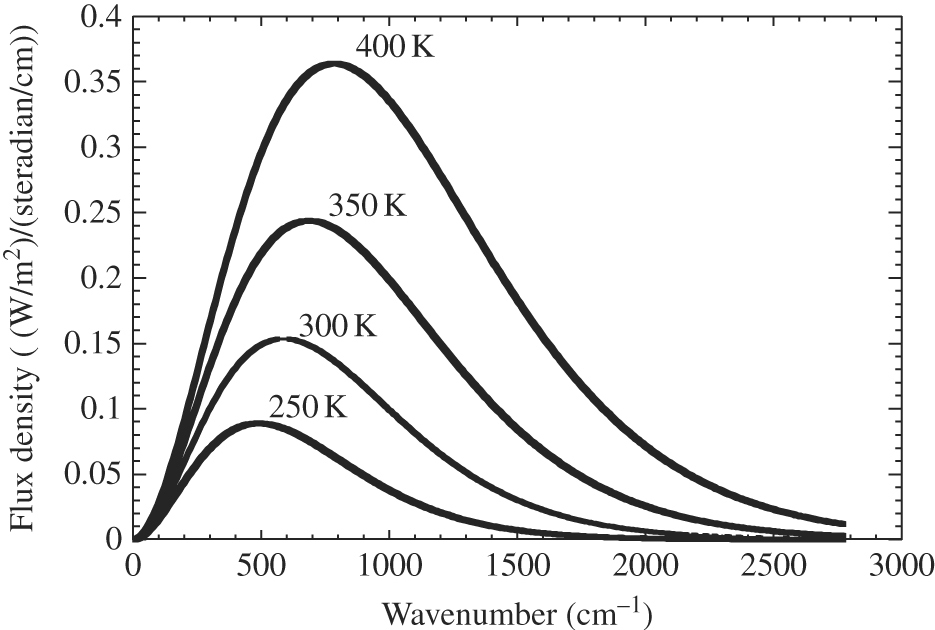
\includegraphics[width=\linewidth]{Figures/Radiative Transfer/BB Spectral Radiance.png}
        \caption{Spectral Radiance $L=B(\nu,T)$ of a Black Body}
        \label{Spec Rad BB}
    \end{subfigure}
    \begin{subfigure}{0.35\linewidth}
        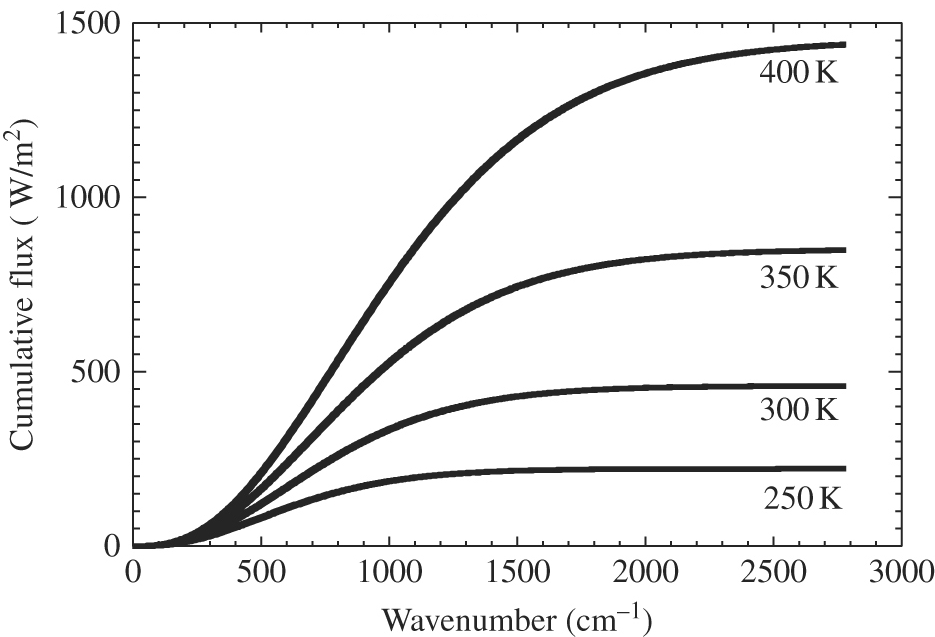
\includegraphics[width=\linewidth]{Figures/Radiative Transfer/BB Cumulative.png}
        \caption{Cumulative Radiance $\int B d\nu$ of a Black Body}
        \label{Cum BB}
    \end{subfigure}
    \begin{subfigure}{0.25\linewidth}
        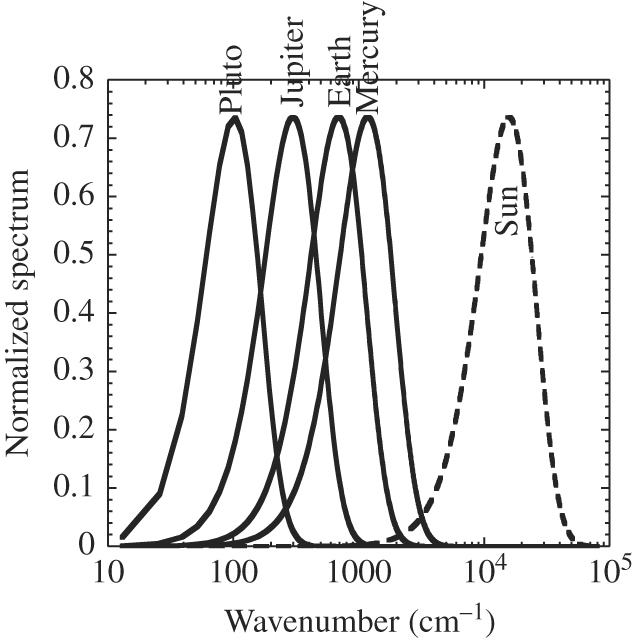
\includegraphics[width=\linewidth]{Figures/Radiative Transfer/Spectral Gap.jpg}
    \end{subfigure}
\end{figure}

Third and finally, $B$ is not a function if $\vec{\omega}$: $B$ is isotropic! This final fact allows us to calculate the spectral irradiance of a blackbody:
\begin{align*}
    F(\nu,T)&=\int_{\Omega_-} B(\nu,T)\,d\Omega_\perp\\
    &= \left( \int_{\Omega_-}d\Omega_{\perp} \right)\,B(\nu,T)\\
    &=\pi B(\nu,T)
\end{align*}

\noindent where we have set the zenith angle $\zeta$ equal to $\theta$ and integrated the projected differential solid angle:
\begin{align*}
    \int_{\Omega_-}d\Omega_\perp&=\int_{\Omega_-} \cos \zeta \,d\Omega\\
    &=\int_{0}^{2\pi}\int_{0}^{\frac{\pi}{2}} \cos \zeta \,d\theta \,\sin\theta \,d\phi\\
    &=2\pi \int_{0}^{\frac{\pi}{2}}\sin\theta\cos\theta\,d\theta\\
    &=2\pi\left[ \frac{1}{2}\sin\theta^2 \right]_0^{\frac{\pi}{2}}\\
    &=\pi
\end{align*}

To find the (non-spectral) irradiance of a black body, we integrate over all frequencies to recover the Stefan-Boltzmann Law governing the power output per unit area $P$ of a black body:
\begin{align}\label{Blackbody Frequency}
    \boxed{P=\sigma T^4=\int_0^\infty \pi B(\nu,T)\,d\nu}
\end{align}
\subsection{Emissivity and Kirchoff's Law}

Many bodies are not like blackbodies at all, even approximately. We thus define the \textbf{emissivity} $\epsilon\in[0,1]$ of an object as follows:
\begin{align}
    \BOX{\epsilon(\nu,T,p)=\frac{L(\nu,T,p)}{B(\nu,T)}}
\end{align}
where $T=$ the temperature and $p=$ the pressure of the object in question. Physically, the emissivity encodes how much the object is like a blackbody at each frequency, temperature, and pressure. For a perfect blackbody, $\epsilon=1$ for all frequencies, temperatures, and pressures. One can show that, in local thermodynamic equilibrium, the emissivity of an object is exactly equal to its absorptivity $\alpha$, where $\alpha$ is (dimensionless) the fraction of spectral radiance absorbed by the material.
\begin{align}
    \boxed{\epsilon(\nu,T,p)=\alpha(\nu,T,p)}
\end{align}

We will use this to derive the \hyperref[Schwarzschild]{Schwarzschild Equation}, which governs radiative transfer in the atmosphere. However, we should note that the derivation assumes local thermodynamic equilibrium. This is a good approximation in most parts of the atmosphere, but fails near the top of the atmosphere.

\subsection{Calulating the Stellar Constant}

To a good approximation, stellar bodies are black bodies. We can estimate the incident (not absorbed) radiative energy flux on the Earth (or any planet) from the Sun (or any star) by approximating that star as black body. The spectral radiance of the sun is approximately $B(\nu,T_{sun})$. We define the \textbf{Stellar Constant} $L_{\star}$ as the incident stellar irradiance. Note that this is different from the \textit{absorbed} stellar power – to obtain that we have to account for albedo (some incident stellar irradiance is reflected) and integrate over area. Let us now calculate $L_{\star}$. We do this by integrating the spectral radiance of the Sun over all frequencies (to obtain the radiance) and over the solid angle of the Sun from Earth (to obtain the irradiance):
\begin{align*}
    L_{\star}=\int _0^\infty \int_{\Omega_{Sun}}B_{sun}(T,\nu)\,d\Omega\,d\nu
\end{align*}

Where $\Omega_{sun}$ denotes the solid angle the sun makes from the Earth. Note that we're integrating over $d\Omega$ here, not $d\Omega_\perp$. The sun is a blackbody, and so emits isotropically, so we can simply integrate out solid angles and use the Stefan-Boltzmann Law:
\begin{align*}
    L_{\star}&=\int _0^\infty \Omega_{Sun}B_{sun}(T,\nu)\,d\nu\\
    &=\Omega_{sun}\,\sigma T_{sun}^4\frac{1}{\pi}
\end{align*}

What is the solid angle of the sun $\Omega_{sun}$ then? We can figure this out by considering a sphere centred on the Earth with a radius equal to the distance between the Earth and the Sun. The total solid angle of the entire sphere is $4\pi$, but the Sun is only occupying a small area on the surface of that sphere. The ratio of the area covered by the sun to the area of the entire sphere is $\pi R_{sun}^2:4\pi R_{Au}$, where $R_{sun}$ is the radius of the sun and $R_{Au}$ is the distance between the sun and the Earth.
\begin{align*}
    \Omega_{sun}&=4\pi\frac{\pi R_{sun}^2}{4\pi R_{Au}^2}\\
    &=\pi \frac{R_{sun}^2}{R_{Au}^2}
\end{align*}

\noindent Therefore:
\begin{align}
    L_{\star}=\frac{R_{sun}^2}{R_{Au}^2}\,\sigma T_{sun}^4
\end{align}

The power actually absorbed by the Earth is given by integrating over area and accounting for reflection. Suppose some fraction $\alpha\in[0,1]$ of the instellation is reflected. Therefore:
\begin{align*}
    P_{in}&=\int (1-\alpha)L_\star \,\cos \zeta\,dA\\
    &=(1-\alpha)L_\star\int \cos \zeta\,dA
\end{align*}

Where we have reintroduced the zenith angle factor $\cos \zeta$ (since we only integrated over $d\Omega$ before rather than $d\Omega_\perp$). This is to represent the fact that the sun is only hitting the Earth from one side, and only the component perpendicular to the ground is absorbed. As such, $\int\cos\zeta\, dA$ is the \textit{projected} area of the Earth due to the $\cos \zeta$ term, and therefore is $\pi R^2$, not $4\pi R^2$. Therefore:

\begin{align}
    P_{in} = (1-\alpha)\pi R^2 \frac{R_{sun}^2}{R_{Au}^2}\,\sigma T_{sun}^4
\end{align}

If we also approximate the Earth as a blackbody, and its radiation as isotropic, we can estimate the outgoing power:
\begin{align*}
    P_{out}&=\int\int_{\Omega_+}\int _0^\infty B(\nu,T_{Earth})\,d\nu\,d\Omega_\perp\,dA\\
    &=\left(\int dA\right)\int_{\Omega_+}\,d\Omega_\perp\int _0^\infty B(\nu,T_{Earth})\,d\nu\\
    &=(4\pi R^2)\,\sigma T_{Earth}^4
\end{align*}

From energy conservation, $P_{in}-P_{out}=0$, which we can solve for the equilibrium temperature of the Earth:
\begin{align*}
    0&=(1-\alpha)\pi R^2 \frac{R_{sun}^2}{R_{Au}^2}\,\sigma T_{sun}^4-(4\pi R^2)\,\sigma T_{Earth}^4 \\
    \therefore 0&=(1-\alpha) \frac{R_{sun}^2}{R_{Au}^2}\, T_{sun}^4-4 T_{Earth}^4 \\ 
    \therefore T_{Earth}&=T_{sun}\left(
    \frac{1-\alpha}{4}\frac{R_{sun}^2}{R_{Au}^2}
    \right)^\frac{1}{4}
\end{align*}

\section{Absorption: Optical Thickness and Transmission Function}

Suppose some spectral radiance is traveling through a slab of radiation-absorbing \textit{stuff} (e.g., air) with an infinitessimal mass-path of $d\mu$, where $d\mu$ is the mass per area (perpendicular to the propogation of radiation). We define the infinitesimal \textbf{Optical Thickness} $d\tau_\nu$ of the slab as the absorptivity $\alpha$ of the slab. In other words, suppose some spectral radiance $L$ is traveling through the radiation-absorbing \textbf{stuff}. Then the infinitesimal change of spectral radiation by the slab $dL$ is given by:
\begin{align*}
    dL &= -\alpha(\nu,T)L\\
    &= d\tau_\nu\,L
\end{align*}
where I have written $\tau_\nu$ with a subscript $\nu$ to remind us that $\tau_\nu$ is a strong function of $\nu$. We further define the absorption cross section $\kappa(\nu,T,p)$ as the effective area of spectral radiance absorbed per unit mass of absorber encountered. $\kappa$ has units of \qty{}{\metre\squared\per\kilogram}, and will generally depend on frequency, temperature, and pressure. Therefore: 
\begin{align}
    \boxed{d\tau_\nu=\kappa(\nu,T,p)\,d\mu}
    \label{Optical Thickness}
\end{align}

We can integrate this between two points in the atmosphere $p_1$ and $p_2$ to find the final spectral radiance $L_{2}$ in terms of the initial spectral radiance $L_{1}$:
\begin{align*}
    \frac{dL}{L}&=-d\tau_\nu\\
    \therefore\int_{p_1}^{p_2}\frac{dL}{L}&=-\left|\int_{p_1}^{p_2}d\tau_\nu\right|\\
    \ln\left( \frac{L_2}{L_1} \right)&=-\left|\int_{p_1}^{p_2}d\tau_\nu\right|\\
    \therefore L_2&=L_1\exp\left(-\left|\int_{p_1}^{p_2}d\tau_\nu \right|\right)
\end{align*}

Notice the absolute value in the second line. If we did not have this, we could simply reverse the limits of integration (e.g., integrate from $p_2$ to $p_1$) and obtain that the spectral radiance \textit{increases} as it passes through. However, this is clearly unphysical: the spectral radiance absorbed should be the same regardless of whether the radiation is going upwards through the absorber or downwards through the absorber. Finally, if we note that:
\begin{align*}
    \tau_\nu(p_1)-\tau_\nu(p_2)=\int_{p_1}^{p_2}d\tau_\nu=\int_{p_1}^{p_2}\kappa(\nu,T,p)\,d\mu
\end{align*}
then we can define the transmission function $\mathcal{T}_\nu$ which encodes the absorption of the spectral irradiance between those two points:
\begin{align}
    \mathcal{T}_\nu(p_1,p_2)=e^{-|\tau_\nu(p_1)-\tau_\nu(p_2)|}
    \\
    L_2=L_1\,\mathcal{T}_\nu(p_1,p_2)\nonumber
\end{align}

Note that it is only the transmission function which is physically and dynamically significant here, as \textit{that} is what determines absorption. We could work directly with the transmission function, but for convenience, we'd much rather work in terms of optical depth.

However, the optical depth itself is not directly physically meaningful. This is because the transmission function only cares about absolute value differences in optical depth.\footnote{
    The situation is analogous to Classical Electromagnetism or Newtonian Mechanics. In Electromagnetism and Mechanics, the only objects of physical consequence are the \textit{forces}, which depend only on the electric/magnetic fields ($\vec{E},\vec{B}$)\footnotemark and accelerations ($\ddot{\vec{r}}$) respectively. However, for convenience, we'd rather work with the electromagnetic scalar/vector potentials ($\phi,\vec{A}$) or  positions ($\vec{r}$), so we have some freedom to choose some properties of ($\phi,\vec{A}$) or ($\vec{r}$). In the former case, we must fix the gauge (e.g., pick the Lorenz or Coulomb gauge) and in the latter case, we must pick the origin and veloctiy of our coordinate system (e.g., pick the origin as the centre of the Earth). In fancy speak, we say that electromagnetism has a gauge symmetry and Newtonian mechanics has galillean symmetry. We must do a similar thing here for optical depth.
}\footnotetext{Actually the situation in electromagnetism is a bit more complicated than I've made it. In fact, only the motion of charged objects is directly observable. Since $\vec{B}$ interacts with matter through equations involve its cross product (the Biot-Savart Law and $\vec{F}=q\vec{v}\times\vec{B}$), we've used a convention of the right-handed cross product ($\vec{x}\times\vec{y}=\vec{z}$). We could have equally used the left handed cross product and had equivalent empirical predictions. I'm also not going to go into bivectors and pseudovectors here, because this footnote is already too long.} As such, we must make two choices when calculating our optical depth (analogous to choosing, e.g., the origin of our coordinate system in Newtonian mechanics):
\begin{enumerate}
    \item It's ordering: we can let $\tau_\nu$ \textit{increase} with height (decrease with pressure) or \textit{decrease} with height (increase with pressure). This is because the transmission function only cares about the absolute values.
    \item The reference value: we can pick $\tau_\nu=\tau_{\nu,ref}$ at any reference level. This is because the transmission function only cares about differences in optical depth.
\end{enumerate}
I will adopt Ray's convention here, although I should note he switches it up for convenience (as he is well within his rights to!) in section \ref{Shortwave}. As such I will choose:
\begin{enumerate}
    \item $\tau_\nu$ to increase with height, i.e., $\tau_\nu$ to decrease with pressure.
    \item $\tau_\nu$ to be equal to $0$ at the ground.
\end{enumerate}

We now specify that the spectral radiance is travelling through a slab of air with some density $\rho$ and with some absorber with mass-fraction $q$. We can see that $d\mu=q\,\rho\,dl$ where $dl$ is the length of atmosphere the radiation travels through. We further specify that the spectral radiance is traveling at some angle $\theta$ relative to the vertical so that $dl=+dz/\cos\theta$ where $z=$ the height\footnote{I could have equally chosen that $dl=-dz/\cos\theta$ here.}. Finally, we relate $dz$ to $dp$ through Hydrostatic Balance (\ref{Hydrostatic Balance}). Then:
\begin{fact}{Optical Depth Coordinates and the Transmission Function}{Optical Depth Box}\label{Optical Depth Box}
    We define the optical depth coordinate $\tau_\nu$, which encodes how much absorbing \textit{stuff} is below a pressure level $p$:

    \begin{minipage}{.5\linewidth}
        \begin{gather}
            \label{Optical Pressure}
            \BOX{d\tau_\nu=-\kappa(\nu,T(p),p)\,q(p)\frac{dp}{g\,\cos\theta}}\\
            \BOX{\tau_\nu=0\text{  at  }p=p_s}
        \end{gather}
    \end{minipage}
    \begin{minipage}{.5\linewidth}
        \begin{gather}
            \BOX{\tau_\nu(p)=\int_{p_s}^p-\kappa(\nu,T(p'),p')\,q(p')\frac{dp'}{g\,\cos\theta}}\\
            \BOX{\tau_{\nu,\infty}=\tau_\nu(0)}
        \end{gather}
    \end{minipage}
    The transmission function $\mathcal{T}_\nu$ between two points $p_1$ and $p_2$ encodes how much the spectral radiance is attenuated between the two points and is:

    \begin{minipage}{.5\linewidth}
        \begin{align}
            \BOX{
                \mathcal{T}_\nu(p_1,p_2)=e^{-|\tau_\nu(p_1)-\tau_\nu(p_2)|}
            }
        \end{align}
    \end{minipage}
    \begin{minipage}{.5\linewidth}
        \begin{align}
            \BOX{
                L(\nu,p_2)=L(\nu,p_1)\,\mathcal{T}_\nu(p_1,p_2)
            }
        \end{align}
    \end{minipage}
\end{fact}

Notice that I write $T=T(p)$ here. Until \ref{Radiative Equilibrium}, we assume that the vertical temperature profile of the atmosphere is given by some known relation (perhaps the \hyperref[Dry Adiabat]{Dry Adiabat} if we are in the troposphere).

\subsection{Example: Grey Atmosphere and Well Mixed Absorber}

Let us make three assumptions. First, assume that the atmosphere is \textit{grey}. This amounts to the assumption that the atmosphere interacts with light in the same way regardless of frequency, so $\frac{\partial\kappa}{\partial\nu}=0$. Second, assume that $\kappa$ has no $T$ or $p$ dependence. Third, assume that the absorber is \textit{well-mixed}. This means that the concentration $q$ is independent of height $\frac{\partial q}{\partial p}=0$. We can now integrate the optical depth to find:
\begin{align*}
    \tau_\nu(p)&=\int_{p_s}^p-\kappa\,q(p)\frac{dp'}{g\,\cos\theta}\\
    &=-\kappa\,q\frac{1}{g\,\cos\theta}\int_{p_s}^pdp'\\
    &=\frac{\kappa \,q}{g\,\cos\theta}(p_s-p)
\end{align*}
We define $\tau_\infty=\int_{p_s}^0d\tau_\nu$ as the optical depth of the \textit{entire} atmosphere (at that angle $\theta$). Therefore:
\begin{align*}
    \tau_\infty&=\tau(0)\\
    &=\frac{\kappa \,q}{g\,\cos\theta}(p_s-0)\\
    &=\frac{\kappa \,q\,p_s}{g\,\cos\theta}\\
    \therefore\tau_\nu(p)&=\tau_\infty\left(1-\frac{p}{p_s}\right)
\end{align*}
However, typically, $\kappa$ is a strong function of $\nu$. We will discuss how exactly $\kappa$ depends on $\nu$ in the next chapter.

\chapter{Molecular Spectroscopy}

\section{Spectral Lines}

Here we cover how the absorption cross section $\kappa$ depends on $\nu$. In almost all cases, save \hyperref[Continuum]{Continuum Absorption}, $\kappa$ is made up of many `spectral lines' (see Figure \ref{CO2 zoomed} and ignore the white lines).
\begin{figure}[H]
    \centering
    \begin{subfigure}{0.4\linewidth}
        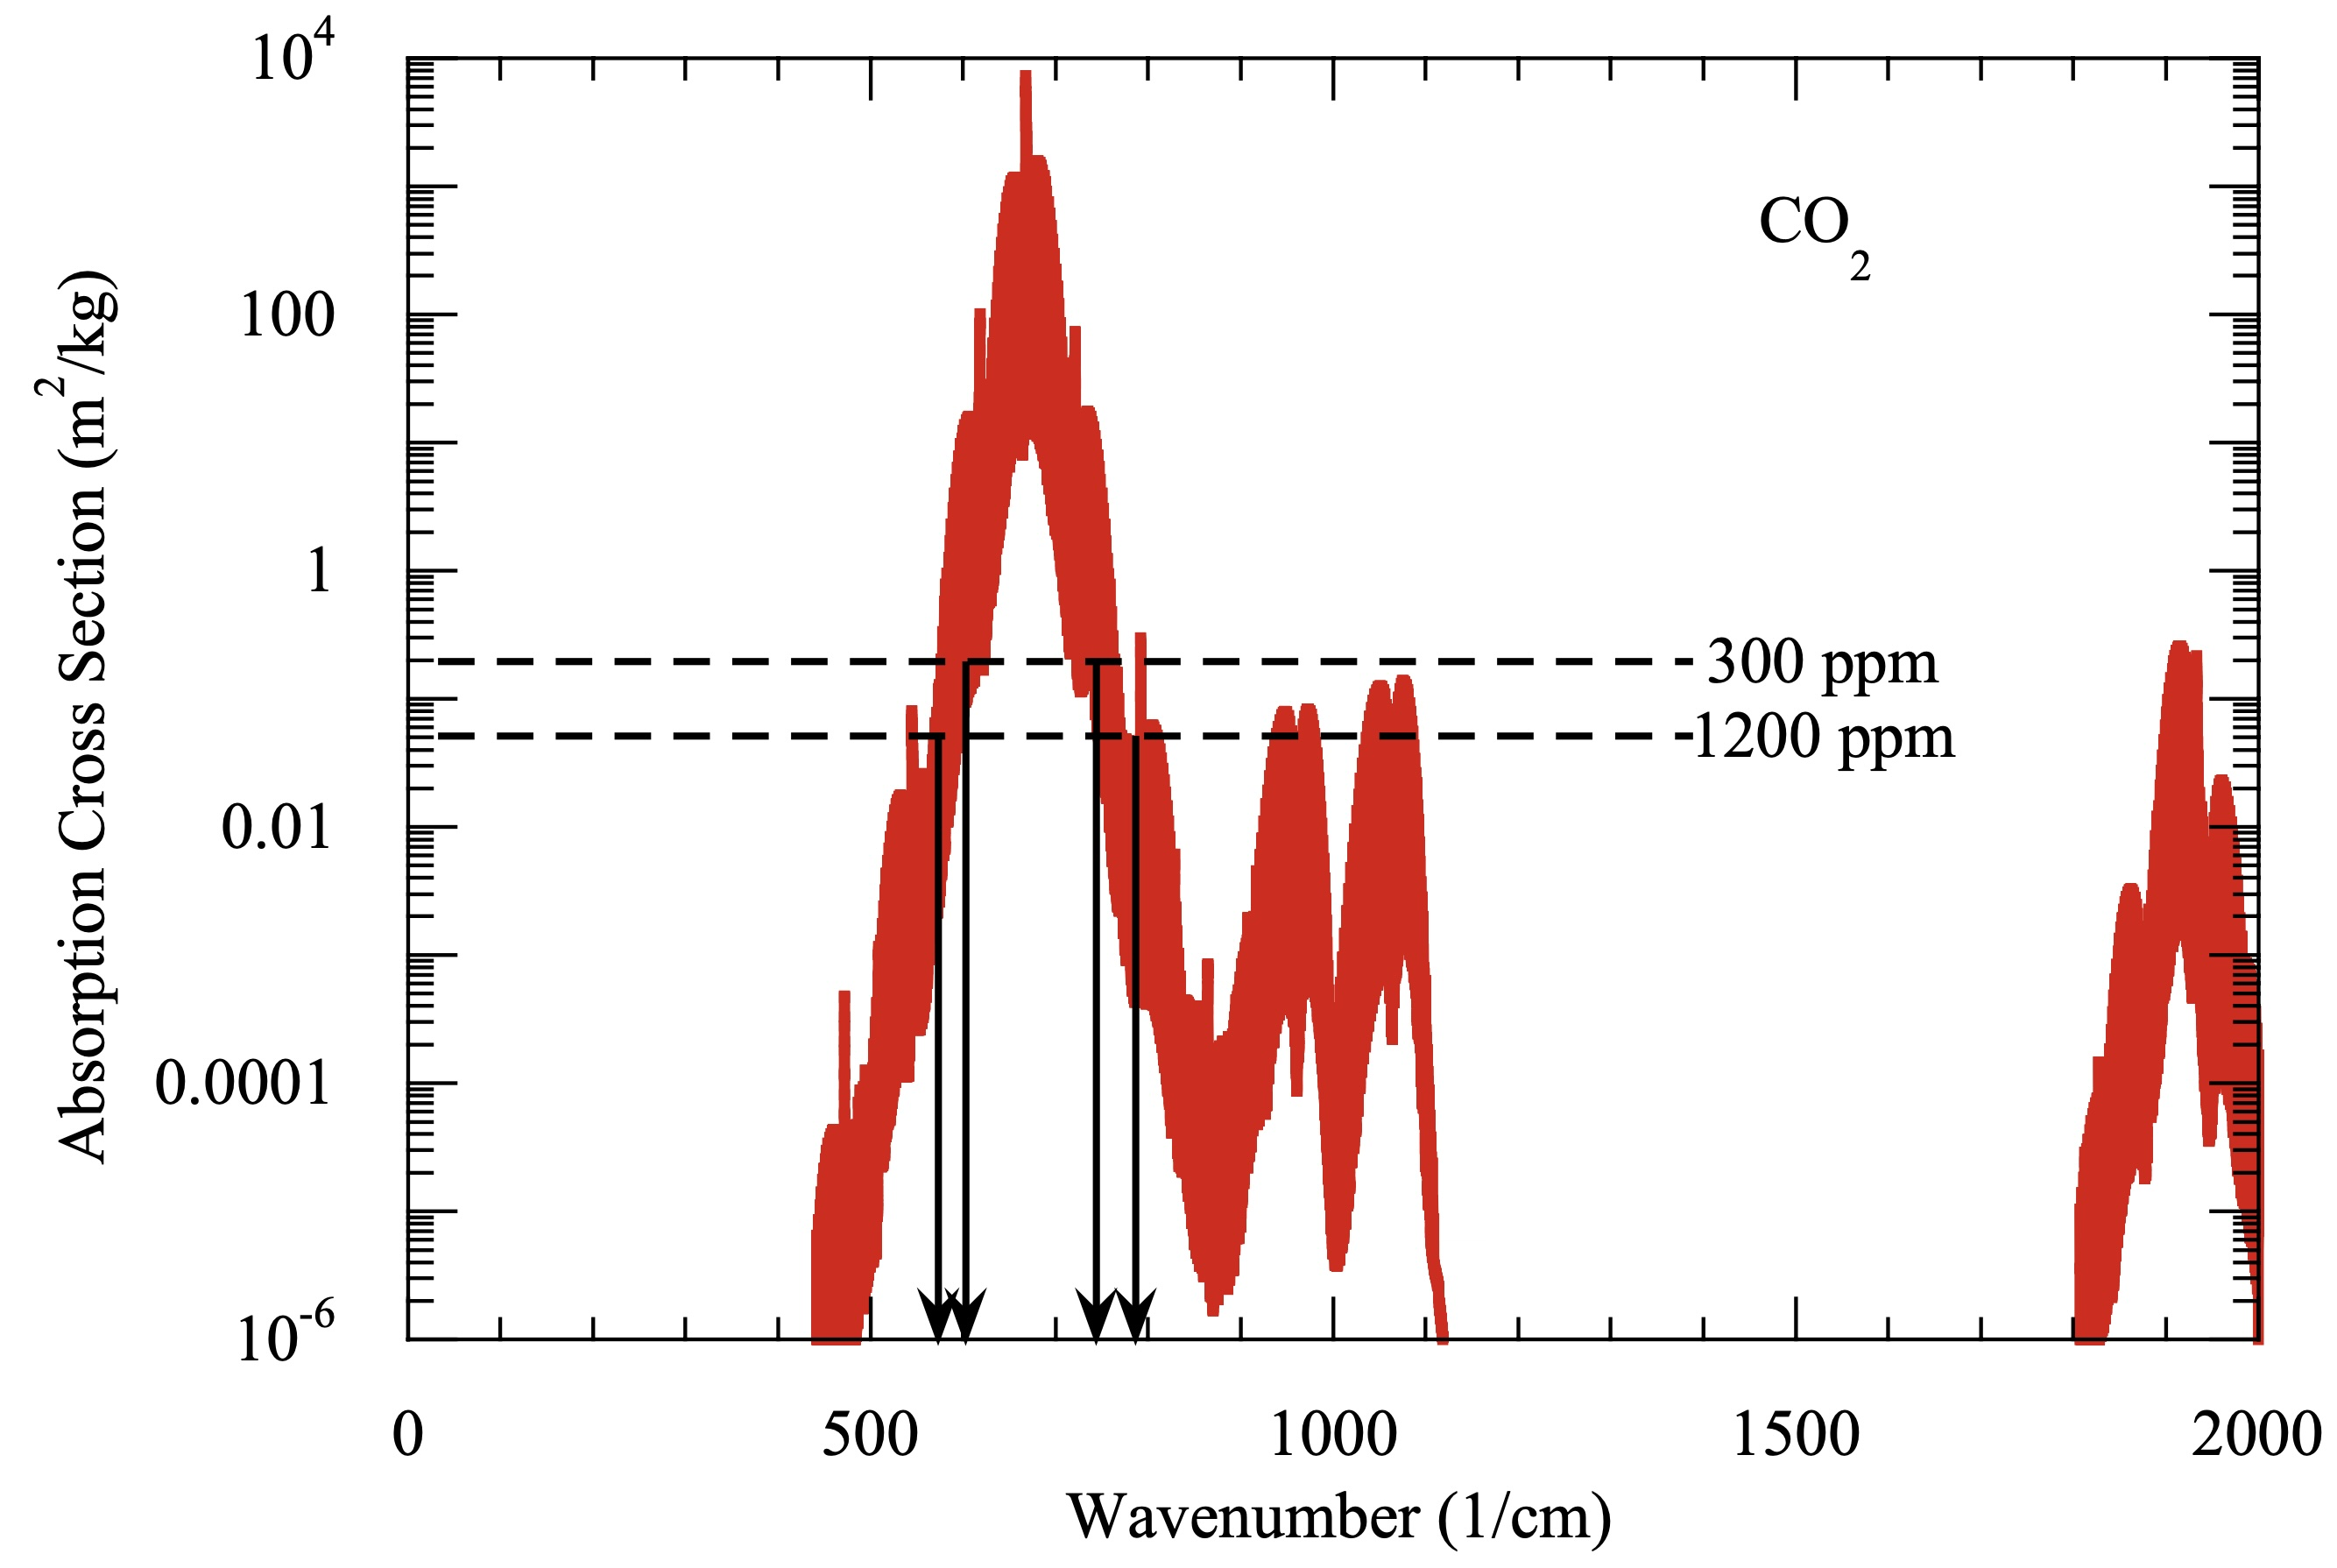
\includegraphics[width=\linewidth]{Figures/Radiative Transfer/CO2 kappa}
        \subcaption{Notice the \textbf{strong} variation over $\nu$ indicated by the logarithmic y-axis scale.}
    \end{subfigure}
    \quad
    \begin{subfigure}{0.4\linewidth}
        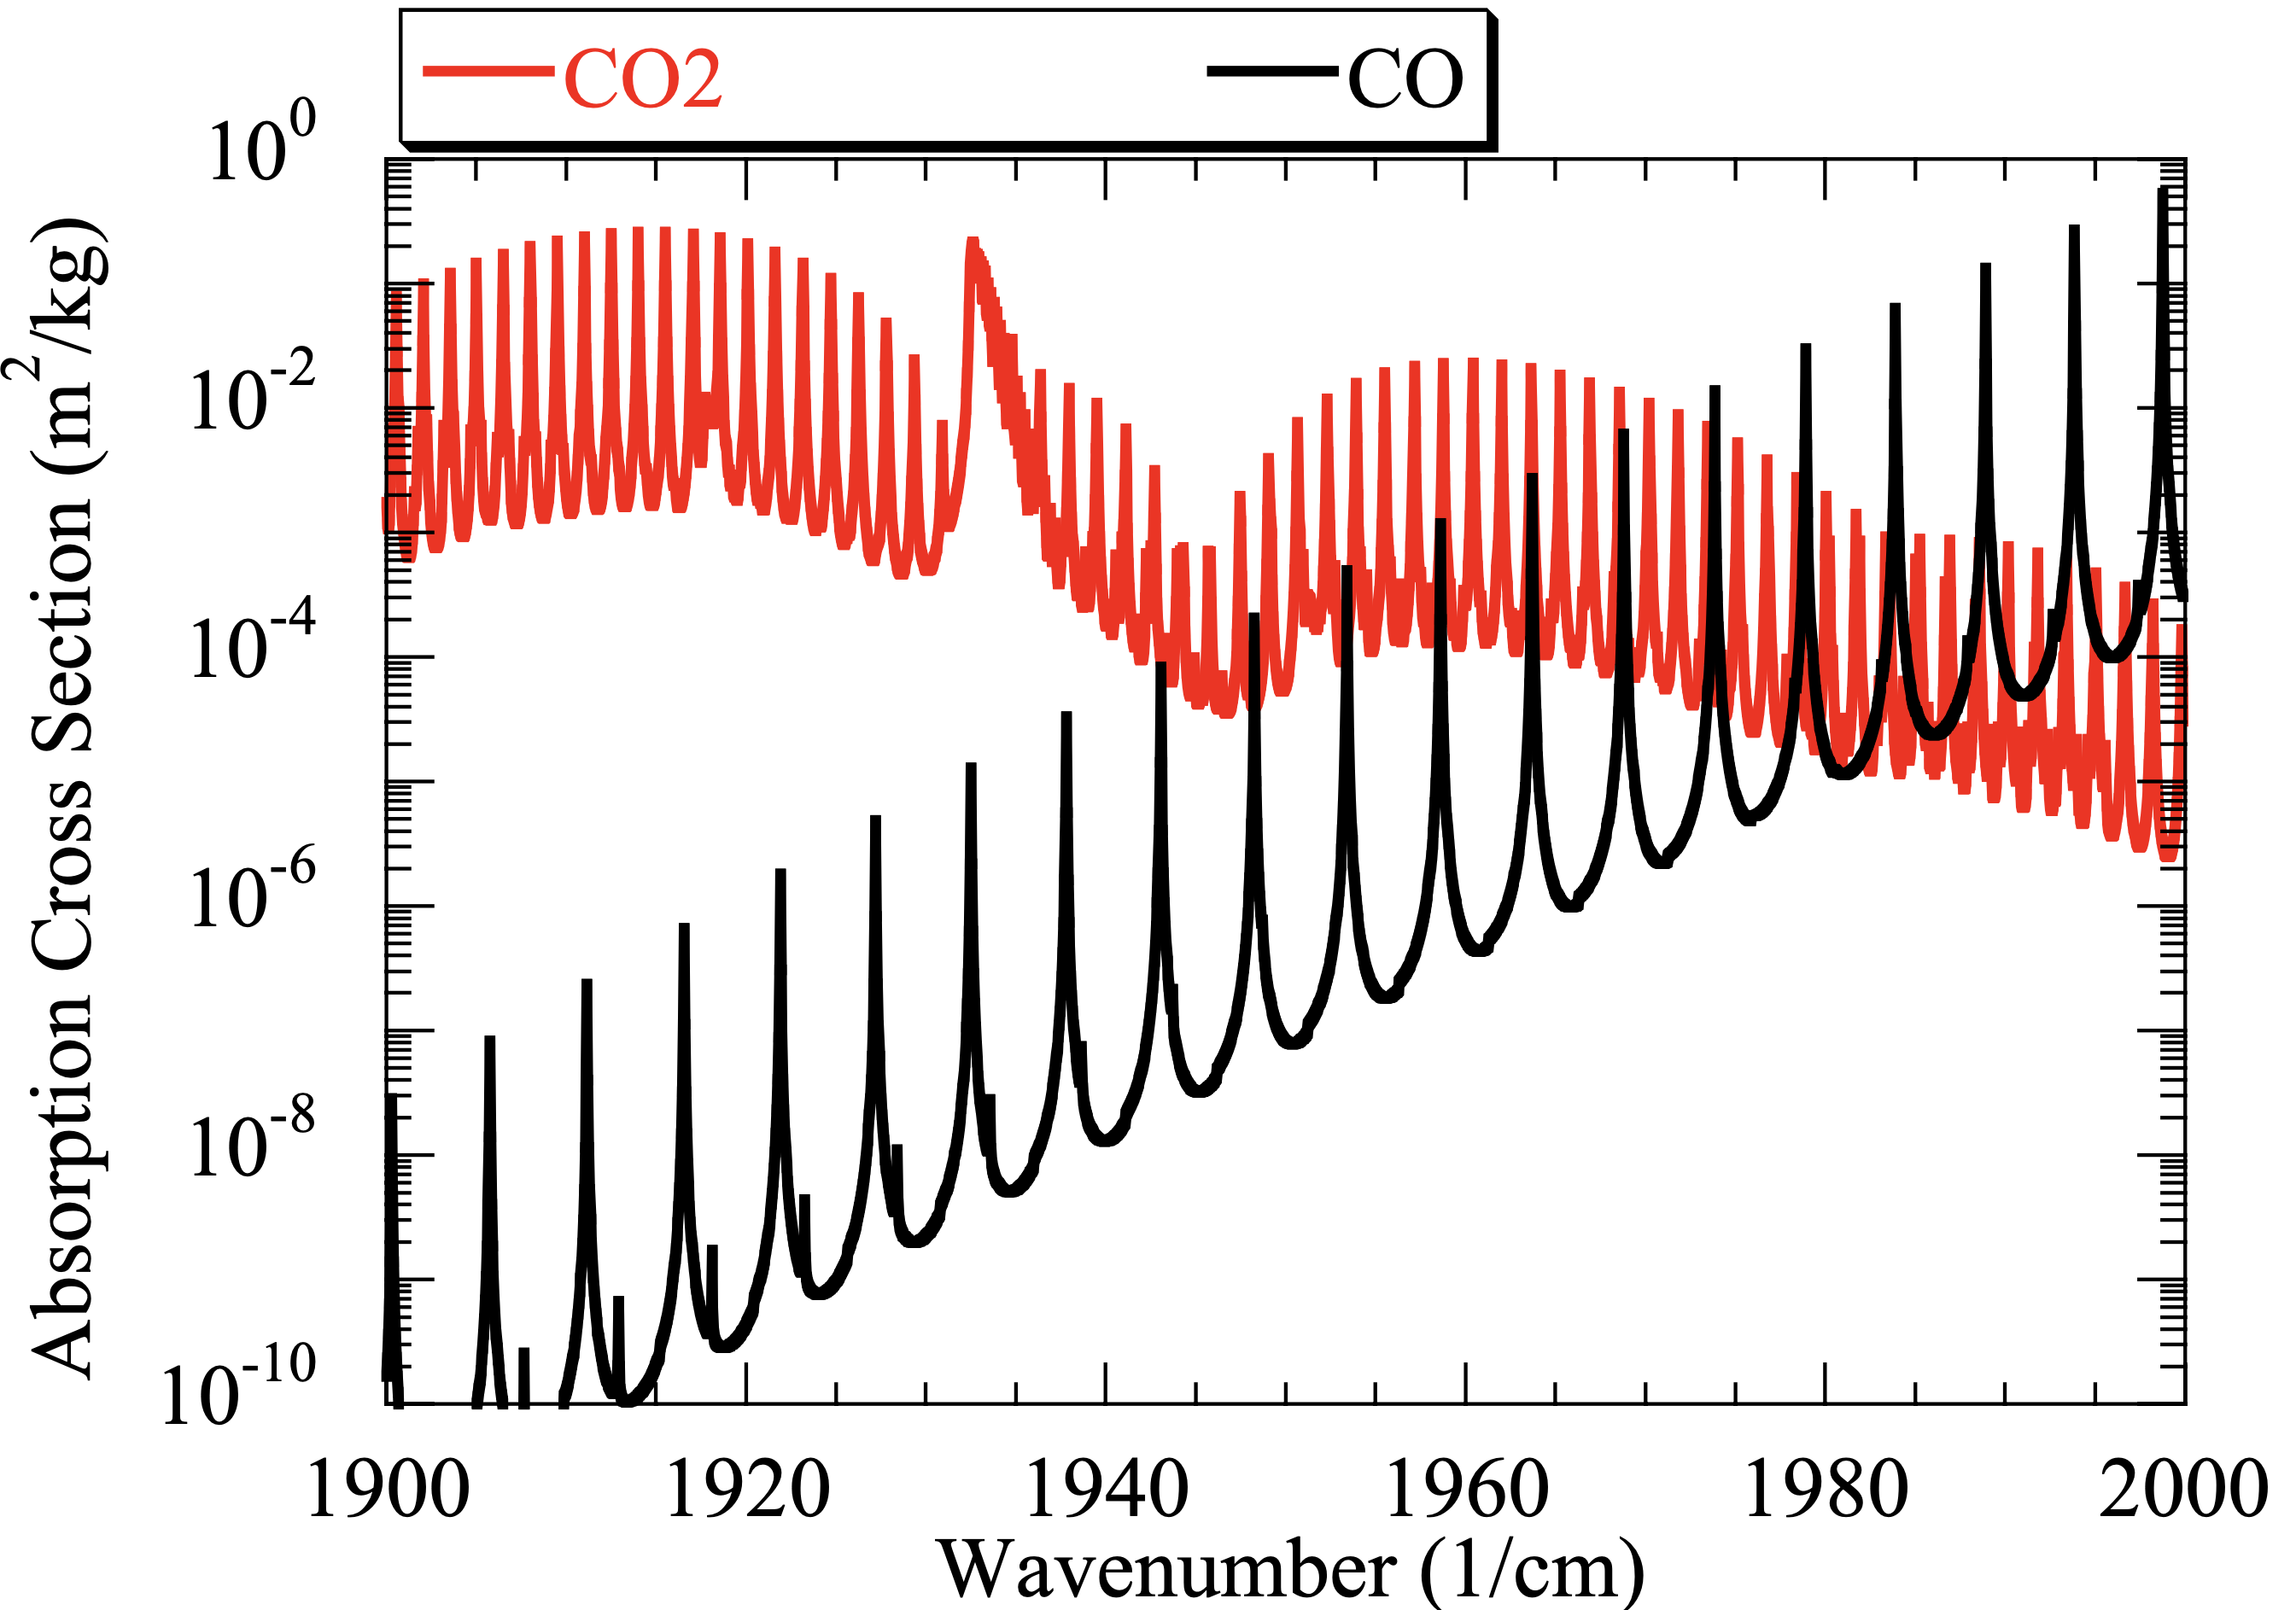
\includegraphics[width=\linewidth]{Figures/Radiative Transfer/CO2 zoomed.png}
        \subcaption{Notice how the curve is made up of \textbf{spectral lines}. }
        \label{CO2 zoomed}
    \end{subfigure}
    \caption{CO$_2$'s Absorption Cross Section at \qty{100}{\milli\bar} and \qty{260}{\kelvin}. Figures from Ray's lecture slides.}
    \label{CO2 kappa}
\end{figure}
We will discuss how to characterise the \textbf{line shape} of each individual spectral line, which we will refer to as $\kappa_{\nu_c}$: 
\begin{fact}{Line Shape}{Line Box}\label{Line Box}
    An individual spectral line is characterised as follows. All parameters have units of \qty{}{\per\second}.
    \begin{align}
        \BOX{\kappa_{\nu_c}(\nu)=\frac{S}{\delta}F\left( \frac{\nu-\nu_c}{\delta} \right)}
    \end{align}
    \begin{minipage}{.45\linewidth}
        \textbf{Line Centre} $\nu_c$:
        encodes the centre of the spectral line.

        \vspace{5 mm}
        \textbf{Line Strength} $S$: encodes how strong of an absorber the spectral line is. Defined as follows:
        \begin{align}\label{Strength}
            S=\int_{-\infty}^{\infty}\kappa(\nu)\,d\nu
        \end{align}
        Generally a function of $T$
    \end{minipage}
    \hfill
    \begin{minipage}{.45\linewidth}
        \textbf{Line Width} $\delta$:
        encodes how wide the spectral line is. Generally a function of $p$ and $T$.
        
        \vspace{5 mm}
        \textbf{Line shape} $F(x)$: encodes the shape of the line (e.g., how does the line decay as $\nu$ goes away from $\nu_c$). Normalised such that:
        \begin{align*}
            \int_{-\infty}^{\infty}F(x)\,dx=1
        \end{align*}
    \end{minipage}
\end{fact}
Why do gases absorb/emit electromagnetic radiation in the first place? Gases absorb/emit electromagnetic radiation because its consitutents, the molecules, have different states corresponding to different energy levels. If a molecule recieves just enough energy from a photon, it can transition from a lower energy level to a higher energy level, and thus absorb the photon. If a molecule is already in a higher energy level, it can spontaneously emit a photon to transition to a lower energy level.

There are three types of transitions that a molecule can undergo:
\begin{enumerate}
    \item \textbf{Electron Transitions}: An electron on the molecule hops to a higher energy state. Typically visible and UV frequency photons cause/are emitted from these transitions.
    \item \textbf{Vibrational Transitions}: The molecule begins vibrating/vibrates faster. Typically IR (Infrared) frequency photons cause/are emitted from these transitions.
    \item \textbf{Rotational Transitions}: The molecule begins rotating/rotates faster. Typically microwave frequency photons cause/are emitted from these transitions.
\end{enumerate}

We will now discuss what determines each parameter of $\nu_c$, $S$, $\delta$ and $F(x)$.

\subsection{Line Centre\texorpdfstring{ $\nu_c$}{}}

In order to discuss what determines the line centre $\nu_c$, we must discuss why spectral lines exist at all, rather than $\kappa$ having a very smooth dependence on $\nu$.

When a molecule absorbs a photon of frequency $\nu$, it must recieve energy $E=h\nu$. However, as discussed in Section \ref{Equipartition}, the energy levels of molecules are quantised, so molecules can only absorb a photon with energy equal to the energy level spacings $\Delta E$. As such, $\nu$ is constrained such that $\nu=\Delta E/h$, and this is what sets the line centre. $\Delta E$ itself is set by the quantum mechanical properties of the molecule, which is found through a variety of empirical and theoretical approaches.

A question you might (rightfully) have now is the following: if energy levels are discritised such that the molecule can only absorb energy of $E_1$, $E_2$, $E_3$, \ldots, then it can only absorb photons with a frequency \textit{exactly} equal to $\nu_1=h/E_1$, $\nu_2=h/E_2$, $\nu_3=h/E_3$, \ldots. Therefore, we should expect $\kappa$ to be a collection of infinitely thin lines, and nothing like what we see in Figure \ref{CO2 kappa}, which is a collection of thin bumps! Furthermore, since only infinitely thin lines are absorbed, then nothing is actually absorbed at all, so $\kappa=0$ for all materials! What went wrong?

This question will be answered when we discuss \hyperref[Broadening]{Broadening Mechanisms}.

\subsection{Line Strength\texorpdfstring{ $S$}{}}

The line strength $S$ is determined by two factors.

The first factor is how strongly the molecule couples with the electromagnetic field. Typically, \textbf{electron} transitions already couple strongly to the electromagnetic field, as electrons are already charged, and moving charges couple strongly to electromagnetic radiation.

For \textbf{vibrational} and \textbf{rotational} transitions, the distortions of the molecule caused by the vibrations or rotations must change the molecules electric \textbf{dipole-moment}. A full explanation of what `\textbf{dipole-moment}' means isn't possible here, but the gist of it is this: a molecule has a dipole moment if it has an uneven distribution of electric charge. For example, if it is positively charged on one end and negatively charged on the other.

H$_2$O has an intrinsic dipole moment, since the electrons in the bonds are more closely bound to the oxygen, and so the oxygen is a little bit negatively charged and the hydrogens are a little bit positively charged. Vibrations and rotations alter this, and this makes H$_2$O a very strong infrared absorber.

CO$_2$ has no intrinsic dipole moment, but it has two vibrational modes (INSERT FIGURE HERE) which alter its dipole moment. This is typical of linear triatomic molecules. As such, it is a strong infrared absorber as well.

Meanwhile, N$_2$ and O$_2$ are both diatomic molecules made up of identical atoms, and so don't couple strongly to the electromagnetic field, since none of the rotational or vibrational modes change the molecules' dipole moment. This is why N$_2$ and O$_2$ are both optically inactive.

The second factor depends on the average occupation of the energy states. The intuition is as follows. Suppose a spectral line has a line centre at $\nu_c$, and thus relies on a transition from energy levels from $E_i$ to $E_j$ (such that $E_j-E_i=h\nu_c$). A gas that has, say, half of its molecules in energy state $E_j$ will have half of its molecules able to absorb a molecule of frequency $\nu_c$, but a gas that has a higher proportion (say, three-quarters) will have a higher proportion of its molecules (say, three-quarters) able to absorb a molecule of frequency $\nu_c$.

The occupation of energy states depends on the temperature of a system, and one can derive this using statistical mechanics. We won't derive it here, but the result for the functional form of $S$ for IR (Infra-red) radiation is as follows:
\begin{align*}
    S(T)=S(T_0)\frac{Q(T_0)}{Q(T)}\left( 
        \frac{1-\exp\left( \frac{-h\nu_c}{k_BT} \right)}{1-\exp\left( \frac{-h\nu_c}{k_BT_0} \right)}\exp\left( 
            -\frac{h\nu_l}{k_B}\left( \frac{1}{T}-\frac{1}{T_0} \right)
         \right)
     \right)
\end{align*}
where $h\nu_l$ is the energy of the lower energy state and $Q(T)$ is some function of $T$ depending on the molecule. You do not need to memorise or understand much of this equation, but it's important to note that the main dependence comes from the exponential terms. $S$ \textbf{strongly} increases with temperature (it has an exponential dependence): as temperature increases, line-strength also increases.

\section{Broadening Mechanisms: Line Shape\texorpdfstring{ $F$}{} and Width\texorpdfstring{ $\delta$}{}}\label{Broadening}

If we stop our discussion here, then we would have a collection of infinitely thin lines,and so $F(x)=\delta(x)$ for all lines, where $\delta$ is the dirac delta function. However, lines are clearly \textbf{broadened} (see Figure \ref{CO2 zoomed}) and are not delta functions. There are three physical mechanisms which explain why lines are broadened in our context, and why molecules may absorb/emit photons with frequency $\nu$ close to $\nu_c$ but not equal to $\nu_c$.

\subsection{Uncertainty Broadening}

One can show, but we won't show it here, that the following relation holds:
\begin{align*}
    Var(\hat{E})\,\tau=h/2
\end{align*}
where $Var(\hat{E})$ is the variance of the energy of the system, $\tau$ is the expected lifetime of the system, and $h$ is Planck's constant. To be perfectly honest, I do not fully understand how this equation arises, and what relation this bears to the Heisenberg Uncertainty Relation other than a superficial resemblance.\footnote{
    The Heisenberg Uncertainty Relation relates the variance in momentum and variance in position of any quantum system. Despite what I see as a superficial resemblance, I will be using the name `Uncertainty Broadening' because that's what it's called in C5 and I don't want to confuse you. If I could choose though, I'd probably use the sometimes-used `Lifetime Broadening' or `Natural Broadening'.
}

Let's now interpret the consequences of the equation on the molecules we're considering. The lifetime of a system $\tau$ encodes how stable the system is. Recall that a molecule is in an `excited' state before emitting a photon or after absorbing a photon. This state is, generally, meta-stable, and thus has a finite lifetime ($\tau\neq\infty$) after which it has a high probability of emitting a photon and transitioning to a lower energy state.

The variance of the energy $Var(\hat{E})$ represents the fact that, because of this, these molecules aren't actually in a state of exact/definite energy (called an energy eigenstate). This means that when a system transitions from one energy state to another energy state, the energy difference can actually be approximately equal to $\Delta E$, with some spread determined by the lifetime of the system $\tau$.

One can determine the line width and shape from these principles more rigourously, but it turns out that in normal atmospheric circumstances this line width is negligible, so we do not discuss this in C5. It will suffice for you simply to know that, regardless of whether the upcoming two broadening mechanisms come into effect, there is some natural Uncertainty Broadening mechanism which ensures that \textit{all} lines have finite width.

\subsection{Doppler Broadening}

Our second broadening mechanism is doppler broadening, and this occurs because the molecules in the gas might be moving away/towards us when they absorb or emit a photon. As such, the photon will be red or blue shifted.

Since the molecules are moving at non-relativistic speeds, the (doppler-shifted) frequency $\nu$ we see is related to the actual linecentre $\nu_c$ by:
\begin{align*}
    \nu=\nu_c+(1+v/c)
\end{align*}
where $c=$ the speed of light and $v=$ the velocity the particle is moving in towards/away us.

The actual line-width is thus fixed by the velocity distribution of the molecules. This is predicted by the Maxwell-Boltzmann Distribution using Kinetic Theory, and so we get that:
\begin{gather}
    \label{Doppler Broadening F}
    \boxed{
        F(x)=\frac{1}{\sqrt{\pi}}e^{-x^2}
    }\\
    \label{Doppler Broadening delt}
    \boxed{
        \delta(T) = \frac{\nu_c}{c}\left( \frac{2k_BT}{m} \right)^{\frac{1}{2}}
    }
\end{gather}
So the line-width is scales as $\sqrt{T}$ – the line gets thicker as the gas gets hotter. Conversely, if the temperature falls to $0$ this equation predicts that the line width would fall to $0$, and so $\kappa(\nu=\nu_c)\to\infty$. However, this never happens, as Uncertainty Broadening maintains a non-zero line width.

This is mechanism of broadening is much more substantial than Uncertainty Broadening, but it is still very thin for two reasons. First, as seen from \ref{Doppler Broadening F}, the line shape is exponential in $x$. As such, $F$ falls off extremley rapidly as $\nu$ moves away from $\nu_c$. Second, as seen from \ref{Doppler Broadening delt}, generally $\delta\ll\nu_c$ since $\left( \frac{2k_BT}{m} \right)^{\frac{1}{2}}\ll c$\footnote{Physically, $\left( \frac{2k_BT}{m} \right)^{\frac{1}{2}}$ is proportional to the mean speed of the molecules.}. However, it is dominant in the stratosphere.

\subsection{Collisional/Pressure Broadening}

In the troposphere, this is by far the most important type of broadening. This arises because the kinetic energy of a molecule is not actually quantised. As such, if a molecule is colliding with another molecule while a photon hits it, it can borrow/give some energy to the other molecule to absorb a photon of slightly different frequency than $\nu_c$.

The broadening thus scales with the frequency of collisions, which depends on the pressure and temperature. This gives us the Lorentz Profile:
\begin{fact}{Lorentz Line Shape}{Lorentz Box}\label{Lorentz Box}
    The shape $F$ and width $\delta$ of a spectral line is, in planetary climate contexts, mainly set by the Lorentz Line shape: 
    \begin{multicols}{2}
    \begin{align}
        \label{Lorenz F}
        \BOX{F(x)=\frac{1}{\pi}\frac{1}{x^2+1}}
    \end{align}

    \vspace{18 mm}
    \begin{align}
        \label{Lorenz width}
        \BOX{
            \delta \approx \delta_0\,\frac{p}{p_0}\left( \frac{T_0}{T} \right)^{n}
        }
    \end{align}
    \end{multicols}
    where $\delta_0$, $p_0$, $T_0$ are all reference widths, pressures, and temperatures and $n$ is a dimensionless constant. All constants are, in practice, found empirically. Oftentimes, $n\approx 1/2$.
\end{fact}
As we can see then, pressure broadening results in pressure \textit{increasing} the line width and temperature \textit{decreasing} the line width. If, for example, the pressure were to fall to $0$ this equation predicts that the line width would fall to $0$, and so $\kappa(\nu=\nu_c)\to\infty$. However, again, this never happens, as Uncertainty Broadening (and Doppler Broadening if $T\neq 0$) would maintain a non-zero line width.

You should memorise this for the exam Key Idea \ref{Lorentz Box} for the exam.

\section{Continuum Absorption}\label{Continuum}

[Under Construction]

\chapter{Schwarzschild Equation}

\section{The Equations of Motion}

Consider some radiation traveling through a slab of atmosphere at some zenith angle $\theta$ with some spectral radiance $L$ with some frequency $\nu$. We wish to derive how $L(\nu)$ varies as it propogates through the atmosphere. Suppose the slab of atmosphere has vertical infintesimal optical thickness of $d\tau_\nu^*$. Since the path of the radiation is slanted, the spectral radiance travels through an infinitesimal optical depth of $d\tau_\nu=d\tau_\nu^*/\cos\theta$. The slab absorbs some spectral radiance, but it also emits some spectral radiance:

\begin{figure}[H]
    \centering
    \begin{tikzpicture}
        \draw[-] (1,0) -- (14,0) -- (14,1) -- (1,1) -- (1,0);
        \draw[<->] (14.5,0) -- (14.5,1);
        \node[] at (16,0.5) {$d\tau_\nu^*=d\tau_\nu\cos\theta$};
        \draw[->,ultra thick] (13,-1) -- (9,0);
        \draw[->,ultra thick,dashed] (9,0) -- (5,1);
        \draw[-] (9,0) -- (9,1);
        \coordinate (C) at (9,1);
        \coordinate (A) at (9,0);
        \coordinate (B) at (5,1);
        \draw (C) -- (A) -- (B)
            pic [draw=black, fill=myorange,angle radius=4mm, opacity=0.5] {angle = C--A--B};
        \draw[<->] (7,0) -- (3,1);
        \node[] at (4,0.5) {$d\tau_\nu$};
        \draw[->,ultra thick] (5,1) -- (1,2);
        \draw[->, ultra thick] (13,1) -- (9,2);
        \node[] at (11.25,1.75) {$B\,d\tau_\nu$}; 
        \node[] at (6,1.75) {$L(\tau_\nu^*)-L(\tau_\nu^*)\,d\tau_\nu$};
        \node[] at (10.75,-0.75) {$L(\tau_\nu^*)$};
        \node[] at (8.5,0.5) {$\theta$};
    \end{tikzpicture}
\end{figure}

The spectral radiance going into the slab is $L(\tau_\nu^*)$. The spectral radiance going out of the slab is $L(\tau_\nu^*+d\tau_\nu^*)$, which we wish to express in terms of $L(\tau_\nu^*)$. We know that some proportion $\alpha$ of $L(\tau_\nu^*)$ is absorbed by the radiation and that this proportion is equal to the absorptivity $\alpha(\nu,T) = d\tau_\nu$. However, we also know that the slab of atmosphere also emits radiation equal to $\epsilon(\nu,T)\,B(\tau_\nu^*)$, where $\epsilon=$ the emissivity. Therefore:
\begin{align*}
    L(\tau_\nu^*+d\tau_\nu^*)&=L(\tau_\nu^*)\underbrace{(1-\alpha)}_{\text{absorption}}+\underbrace{\epsilon B(\tau_\nu^*)}_\text{emission}\\
    &=L(\tau_\nu^*) - L(\tau_\nu^*)\,d\tau_\nu + \epsilon B(\tau_\nu^*)
\end{align*}
We now assume that the slab is in local thermodynamic equilibrium, and so $\epsilon=\alpha=d\tau_\nu$ and rearrange to get:
\begin{align*}
    \frac{L(\tau_\nu^*+d\tau_\nu^*)-L(\tau_\nu^*)}{d\tau_\nu}=-L(\tau_\nu^*)+B(\tau_\nu^*)
\end{align*}
Inconveniently, our coordinate $d\tau_\nu$ depends on $\theta$, but we wish to have a coordinate be the same at every horizontal position. We thus define $d\tau_\nu^*=d\tau_\nu\cos\theta$ and derive the \textbf{Schwarszchild Equation}:
\begin{align}\label{Schwarzschild}
    \BOX{
        \cos(\theta)\frac{dL}{d\tau_\nu^*}(\tau_\nu^*)=-L(\tau_\nu^*)+B(\nu,T(\tau_\nu^*))
    }
\end{align}

\section{Angle Averaging: The Two-Stream Approximation}\label{Two Stream Approximation}

Note that generally, $L$ is a function of direction ($\frac{\partial L}{\partial \vec{\omega}}\neq0$). We proceed by making what's called the \textit{Two-Stream Approximation}, but we need not make this approximation if we were coding up a full radiative transfer model. We only assume this here to make analytical progress in order to gain some physical intuition.

We define the net upwards and downward fluxes of irradiance as follows:
\begin{align}
    F_+&=\int_{\Omega_+}L(\vec{\omega})\,d\Omega_\perp \\
    F_-&=-\int_{\Omega_-}L(\vec{\omega})\,d\Omega_\perp 
\end{align}

Note that Ray refers to these as $I_+$ and $I_-$ in his notes. However, we shall refer to them here by the letter $F$, because these are (spectral) \textbf{irradiances}, \textbf{not} (spectral) \textbf{radiances}, as we have integrated over solid angles here. We then integrate Equation \ref{Schwarzschild} in the upwards and downwards directions, and make the assumption that $B$ is isotropic.
\begin{align*}
    \int_{\Omega_+}\cos(\theta)\frac{dL}{d\tau_\nu^*}\,d\Omega&=\int_{\Omega_+}-L+B\,d\Omega\\
    \int_{\Omega_+}\frac{dL}{d\tau_\nu^*}\,d\Omega_\perp&=-\int_{\Omega_+}L\,d\Omega+\int_{\Omega_+}B\,d\Omega\\
    \frac{dF_+}{d\tau_\nu^*}&=-\int_{\Omega_+}L\,d\Omega+2\pi B
\end{align*}

So far, everything is roughly very accurate. We now make the \textit{Two-Stream Approximation} in order to relate $F_+$ to $\int_{\Omega_+}L\,d\Omega$. We make (counter-intuitively) the assumption that $L(\vec{\omega})$ is roughly isotropic enough to be pulled outside of the integral over solid angle. This allows us to find that:
\begin{align*}
    \int_{\Omega_+}L\,d\Omega&\approx L\int_{\Omega_+}\,d\Omega \\
    & = L\,2\pi \\
    & = 2\pi \,L \frac{\int_{\Omega_+}\,d\Omega_\perp}{\int_{\Omega_+}\,d\Omega_\perp} \\
    & \approx 2\pi \frac{\int_{\Omega_+}L\,d\Omega_\perp}{\int_{\Omega_+}\,d\Omega_\perp} \\
    & = 2\pi \, \frac{F_+}{\pi}\\\int_{\Omega_+}L\,d\Omega & \approx 2F_+
\end{align*}
We can go through a similar reasoning with $F_-$, which allows us to derive the angle-averaged upwards and downwards Schwarszchild Equations:
\begin{align}
    \label{Upwards Schwarszchild Initial}
    {\frac{1}{2}\frac{dF_+}{d\tau_\nu^*}=-F_++\pi B}\\
    \label{Downwards Schwarszchild Initial}
    {-\frac{1}{2}\frac{dF_-}{d\tau_\nu^*}=-F_-+\pi B}
\end{align}

Note the extra $-$ sign on Equation \ref{Downwards Schwarszchild Initial}. Comparing \ref{Upwards Schwarszchild Initial} with \ref{Schwarzschild}, we can conclude that this approximation is equivalent to setting $\cos(\theta)=\frac{1}{2}$ on average! With this in mind, we define the effective propagation angle $\tilde{\theta}$ as $\tilde{\theta}=\cos^{-1}(1/2)$. We now abuse notation and define $\tau_\nu\equiv \tau_\nu^*/\cos(\tilde{\theta})=2\tau_\nu^*$ to get rid of that pesky $\frac{1}{2}$ factor to obtain the: 
\begin{fact}{Angle-Averaged Schwarzschild Equations}{Schwarz box}\label{Scharz box}
    \begin{gather}
        \label{Upwards Schwarzschild}
        \BOX{\frac{dF_+}{d\tau_\nu}(\tau_\nu)=-F_+(\tau_\nu)+\pi B}
        \\
        \label{Downwards Schwarzschild}
        \BOX{-\frac{dF_-}{d\tau_\nu}(\tau_\nu)=-F_-(\tau_\nu)+\pi B}
    \end{gather}
    We can relate $\tau_\nu$ back to pressure coordinates by using \ref{Optical Pressure}:
    \begin{align}
        d\tau_\nu&=-\kappa(\nu,T(p),p)\,q(p)\frac{dp}{g\frac{1}{2}}\\
        &=-\kappa(\nu,T(p),p)\,q(p)\frac{dp}{g\cos\tilde{\theta}}
    \end{align}
\end{fact}


\section{General Solutions}

We can integrate \ref{Upwards Schwarzschild} and \ref{Downwards Schwarzschild} using an integrating factor and a single boundary condition to find:
\begin{align}
    F_+(\nu,\tau_\nu)=F_+(\nu,0)e^{-\tau_\nu}+\int_0^{\tau_\nu}\pi B(\nu,T(\tau_\nu'))e^{-(\tau_\nu-\tau_\nu')}\,d\tau_\nu' \label{Upwards Soln}\\ 
    F_-(\nu,\tau_\nu)=F_-(\nu,\tau_{\nu,\infty})e^{-(\tau_{\nu,\infty}-\tau_\nu)}+\int_{\tau_\nu}^{\tau_{\nu,\infty}}\pi B(\nu,T(\tau_\nu'))e^{-(\tau_\nu'-\tau_\nu)}\,d\tau_\nu' \label{Downwards Soln}
\end{align}
where we have used the boundary conditions:
\begin{align*}
    \text{at }\tau_\nu=0\text{ , } F_+(\nu,\tau_\nu)=F_+(\nu,0)\\
    \text{at }\tau_\nu=\tau_{\nu_\infty}\text{ , } F_-(\nu,\tau_\nu)=F_-(\nu,\tau_{\infty})
\end{align*}

There are three subtleties we should note. First, note the sign flips between \ref{Upwards Soln} and \ref{Downwards Soln}, arising due to the sign flip on the derivative in \ref{Upwards Schwarzschild} and \ref{Downwards Schwarzschild}. Second, note that the limits of integration are swapped between \ref{Upwards Soln} and \ref{Downwards Soln}, arising due to the difference in boundary conditions.

The final subtlety is the most important: in general $\tau_\nu=\tau_\nu(\nu)$. Suppose we wish to the total radiative upwards flux of energy at some height/pressure level. We cannot simply find $F_+(\tau=\tau(p))$ then integrate over all frequencies, as in general $\tau_{\nu_1}(p)\neq\tau_{\nu_2}(p)$.

Physically, the solution is intuitive: the total upwards radiance at some optical depth $\tau$ is simply the sum of the irradiance at each level $\tau'$, each attenuated by the transmission function between $\tau$ and $\tau'$. To be more explicit, we sum:
\begin{enumerate}
    \item $F_+(\nu,0)e^{-\tau_\nu}$: The irradiance ($F_+(\nu,0)$) from the bottom ($\tau_\nu=0$) of the atmosphere, attenuated by the optical depth $e^{-(\tau_\nu-0)}$.\footnote{Generally, this is the upwards irradiance emitted by the ground on a rocky planet, but one could also choose $\tau_\nu=0$ in the middle of the atmosphere (as you must on a gaseous planet), in which case $F_+(\nu,0)$ will be the total upwards irradiance at that level (originating from all the atmosphere (and ground) underneath it).}
    \item $\pi B(\nu,T(\tau_\nu'))\,d\tau_\nu'\,e^{-(\tau_\nu-\tau_\nu')}$: The irradiance ($B(\nu,T(\tau_\nu'))\,d\tau_\nu'$) from each layer ($\tau_\nu=\tau_\nu'$), also attenuated by the optical depth $e^{-(\tau_\nu-\tau_\nu')}$
\end{enumerate}
The \textbf{Outgoing Longwave Radiation} $OLR$ (in spectral irradiances) is then defined as $F_+(\nu,p=0)=F_+(\nu,\tau=\tau_{\nu,\infty})$ and given by:
\begin{align}
    OLR=F_+(\nu,0)e^{-\tau_{\nu,\infty}}+\int_0^{\tau_{\nu,\infty}}\pi B(\nu,T(\tau_\nu'))e^{-(\tau_{\nu,\infty}-\tau_\nu')}\,d\tau_\nu' \label{OLR Soln}
\end{align}
The physical interpretation is identical. The total upwards spectral radiance escaping is the spectral radiance from each level attenuated by the amount of absorption in between those levels. 

Since the attenuation is exponential, this gives us an optical depth `lengthscale' set by when $(\tau_{\nu,\infty}-\tau_\nu')\sim 1$. We thus define $\tau_{rad}$ as satisfying $(\tau_{\nu,\infty}-\tau_{\nu,rad})= 1$. Anything with radiation coming from an optical depth $\tau_\nu<\tau_{\nu,rad}$ will 


We can rewrite this in terms of the transmission function $\mathcal{T}_\nu(p_1,p_2)$ if we find the differential of the transmission function with respect to $p_2$ and assume that $\tau_\nu(p_1)>\tau_\nu(p_2)$:
\begin{align*}
    d\left( \mathcal{T}_\nu(p_1,p_2) \right)&=d\left( e^{-|\tau_\nu(p_1)-\tau_\nu(p_2)|} \right)\\
    &=e^{-\tau_\nu(p_1)} d\left(e^{\tau_\nu(p_2)} \right)\\
    &= e^{-\tau_\nu(p_1)}e^{\tau_\nu(p_2)}d\tau_\nu(p_2) \\
    &=e^{-|\tau_\nu(p_1)-\tau_\nu(p_2)|}d\tau_\nu(p_2)\\
    \therefore\,\,d\mathcal{T}_\nu(p_1,p_2)&=\mathcal{T}_\nu(p_1,p_2)\,d\tau_\nu(p_2)
\end{align*}


\begin{fact}{Solution to the Angle-Averaged Schwarszchild Equations}{Soln Schwarszchild Box}\label{Soln Schwarszchild Box}
    The total upwards $F_+(\nu,p)$ and downwards $F_-(\nu,p)$ spectral irradiance at frequency $\nu$ and pressure level $p$ is given by the following:
    \begin{gather}
        \label{Upwards Transmission Soln}
        \BOX{F_+(\nu,p)
        =
        F_+(\nu,0)\mathcal{T}_\nu(p,p_s)
        +
        \int_{p'=p_s}^{p}\pi B(\nu,T(p'))\,d\mathcal{T}_\nu(p,p')} 
        \\ 
        \label{Downwards Transmission Soln}
        \BOX{F_-(\nu,p)
        =
        F_-(\nu,0)\mathcal{T}_\nu(0,p)
        +
        \int_{p}^{0}\pi B(\nu,T(p'))e^{-(\tau_\nu'-\tau_\nu)}\,d\tau_\nu' }
    \end{gather}
    where $d\mathcal{T}_\nu(p_1,p_2)=\mathcal{T}_\nu(p_1,p_2)d\tau_\nu(p_2)$ is the differential transmission function with respect to $p_2$. 

    The \textbf{Outgoing Longwave Radiation} $OLR$ (in spectral irradiances) is then defined as $F_+(\nu,p=0)=F_+(\nu,\tau=\tau_{\nu,\infty})$ and given by:
    \begin{align}
        \BOX{OLR=
        F_+(\nu,0)\mathcal{T}_\nu(0,p_s)
        +
        \int_{p_s}^{0}\pi B(\nu,T(p'))\,d\mathcal{T}_\nu(p',p_s) }\label{OLR Transmission Soln}
    \end{align} 
\end{fact}

\section{Frequency Bands}\label{Frequency Bands}

We're not finished yet! Recall that we have expressed $OLR$ in terms of \textit{spectral} irradiances, but we require the (non-spectral) irradiances if we wish to compute the total outgoing radiative energy flux. What we may do now is integrate the $OLR$ over the centre of a single absorption band centred about $\nu_c$. Typically, both $F_+(\nu,0)$ and $B(\nu,T)$ are roughly constant as a function of $\nu$ compared to $\tau_\nu$, so we can treat $F_+(\nu,0)\approx F_+(\nu_c,0)$ and $B(\nu)\approx B(\nu_c)$ for $\nu\in[\nu_c-\frac{\Delta}{2},\nu_c+\frac{\Delta}{2}]$.

Integrating \ref{OLR Transmission Soln} over frequency, we find the following:
\begin{align}
    \BOX{OLR_{\nu_c}
    =
    F_+(\nu_c,0)\bar{\mathcal{T}_{\nu_c}}(0,p_s)
    +
    \int_{p_s}^{0}\pi B(\nu_c,T(p'))\,d\bar{\mathcal{T}_{\nu_c}}(p',p_s)} \label{OLR Transmission Band Soln}
\end{align}
where we have assumed that $\mathcal{T}_{\nu}\approx 0$ at $\nu=\nu_c\pm\frac{\Delta}{2}$ (the line is thin) and defined the \textbf{Band Integrated Transmission Function} $\bar{\mathcal{T}_{\nu_c}}$ as:
\begin{align}\label{Transmission Function Band}
    \bar{\mathcal{T}_{\nu_c}}(p_1,p_2)&=\int_{-\infty}^{\infty}{\mathcal{T}_{\nu}}\,d\nu\\
    &\approx\int_{\nu_c-\frac{\Delta}{2}}^{\nu_c+\frac{\Delta}{2}}{\mathcal{T}_{\nu}}\,d\nu
    \\
    &=\int_{\nu_c-\frac{\Delta}{2}}^{\nu_c+\frac{\Delta}{2}} e^{|\tau_\nu(p_1)-\tau_\nu(p_2)|}\,d\nu
\end{align}

\noindent Note that $OLR_{\nu_c}$ has dimenions of an irradiance (power per area),since $\bar{\mathcal{T}_{\nu_c}}$ has dimensions of frequency and $F_+$ and $\pi B$ have dimensions of spectral irradiance (power per area per frequency). We now abuse notation and write the total $OLR$ as the total power leaving the Earth per unit area. If we assume that the spectral lines don't overlap then we can find $OLR$ by summing up $OLR_{\nu_c}$ for each spectral line centred about each $\nu_c$:
\begin{align*}
    OLR = \sum_{\nu_c} OLR_{\nu_c}
\end{align*}

Now that our $OLR$ is in terms of known quantities and $\bar{\mathcal{T}_{\nu_c}}$, our next goal is to calculate the $\bar{\mathcal{T}_{\nu_c}}$. Typically, this can be done numerically, but to make analytical progress we will look at three cases: the no-line limit, weak line limit, and strong line limit.

\subsection{The No-Line Limit}
I should make you aware that this is my own personal addition and not talked about in the lecture notes. This limit is a bit non-sensical\footnote{
    I think it's non-sensical because optical depth coordinates mkae no sense if $\kappa=0$. Recall that $d\tau\sim \kappa$, so if $\kappa=0$ then $\tau(p)=0$ for all $p$. That being said, our solution still makes sense.
}, but I think it builds some intuition.

The no-line limit is if $\kappa=0$ at that frequency band, and so $|\tau_\nu(p_1)-\tau_\nu(p_2)|=0$. As such, the transmission function $\mathcal{T}_{\nu}(p_1,p_2)=e^{-|\tau_\nu(p_1)-\tau_\nu(p_2)|}=1$ and so:
\begin{align*}
    \bar{\mathcal{T}_{\nu_c}}(p_1,p_2)&=\int_{\nu_c-\frac{\Delta}{2}}^{\nu_c+\frac{\Delta}{2}} 1 \,d\nu\\
    &=\Delta
\end{align*}
We can therefore substitute $\Delta$ for $\bar{\mathcal{T}_{\nu_c}}$ everywhere. Physically, this means that \textit{nothing} is absorbed out of this absorption band: everything in the band from $\nu=\nu-\frac{\Delta}{2}$ to $\nu=\nu+\frac{\Delta}{2}$ is let through. Substituting explicitly that $\bar{\mathcal{T}_{\nu_c}}(p_1,p_2)=\Delta$ and $d\bar{\mathcal{T}_{\nu_c}}(p_1,p_2)=0$ for all , our solution is:
\begin{align*}
    OLR_{\nu_c}=F_+(\nu_c,0)\Delta
\end{align*}
In other words, the $OLR_{\nu_c}$ at this frequency $\nu_c$ is simply set by the upward radiative flux at frequency $\nu_c$ from the ground, Physically, this corresponds to the fact that the atmosphere is completely transparent at this frequency, and so the $OLR_{\nu_c}$ is set only by the ground's properties, and completely ignorant of atmospheric properties such as the concentration of the molecules (which are transparent at this frequency $\nu_c$).

We'll find that in the weak and strong line limits (and indeed in all cases where $\kappa\neq0$) that $\bar{\mathcal{T}_{\nu_c}}<\Delta$, and so the effective `width' will be smaller than $\Delta$, representing the chunk of radiation that is absorbed by the fact that $\kappa\neq0$.

\subsection{The Weak Line Limit}

The weak line limit obtains if $|\tau_\nu(p_1)-\tau_\nu(p_2)|\ll 1$ for all frequencies $\nu$. If $\tau(p)$ is well-behaved, this will be arbitrarily satisfied if $p_1$ and $p_2$ are sufficiently close. We can then Taylor Expand $e^{|\tau_\nu(p_1)-\tau_\nu(p_2)|}$ and keep only first order terms:
\begin{align*}
    e^{-|\tau_\nu(p_1)-\tau_\nu(p_2)|}\approx1-|\tau_\nu(p_1)-\tau_\nu(p_2)|
\end{align*}
We can now integrate over frequencies to find that:
\begin{align*}
    \bar{\mathcal{T}_{\nu_c}}(p_1,p_2)&\approx\int_{\nu_c-\frac{\Delta}{2}}^{\nu_c+\frac{\Delta}{2}} e^{-|\tau_\nu(p_1)-\tau_\nu(p_2)|}\,d\nu\\
    &\approx\int_{\nu_c-\frac{\Delta}{2}}^{\nu_c+\frac{\Delta}{2}} 1-|\tau_\nu(p_1)-\tau_\nu(p_2)|\,d\nu\\
    &=\Delta-\int_{\nu_c-\frac{\Delta}{2}}^{\nu_c+\frac{\Delta}{2}}
    \left|
        \int_{p_2}^{p_1}-\kappa(\nu,T(p),T)\,q(p)\frac{dp}{g\cos\tilde{\theta}}
    \right|
    \,d\nu
    \\
    &=\Delta-
    \frac{1}{g\cos\tilde{\theta}}
    \biggl|
        \int_{p_2}^{p_1}q(p)
        \biggl(\underbrace{ 
            \int_{\nu_c-\frac{\Delta}{2}}^{\nu_c+\frac{\Delta}{2}}\kappa(\nu,T(p),p)
            \,d\nu
            }_{S(T(p))}
        \biggr)
        \,dp
    \biggr|
    \\
    &=\Delta-S(T_0)\left( \frac{1}{g\cos\tilde{\theta}}\left|\int_{p_1}^{p_2}\frac{S(T(p))}{S(T_0)}q(p)\,dp\right| \right)
\end{align*}
The keen reader will note that this result \textbf{differs} from the result obtains in Ray's lecture slides. I am confident, however, that this expression is correct, as this is the expression that shows up in Ray's book \cite{Ray} and the algebra is more rigourous.

We now define (what seems to me as a dodgy definition!) $S(T_0)$ such that:
\begin{align}
    \int_{p_1}^{p_2}\frac{S(T(p))}{S(T_0)}q(p)\,dp\equiv
    \int_{p_1}^{p_2}q(p)\,dp
\end{align}
This means that the band-integrated transmission function in the weak line limit is:
\begin{align}
    \BOX{
        \bar{\mathcal{T}_{\nu_c}}(p_1,p_2)\approx\Delta-S\mu
    }
\end{align}
where 
\begin{align*}
    \mu=\frac{1}{g\cos\tilde{\theta}}\left|\int_{p_1}^{p_2}q(p)\,dp\right|
\end{align*}
is the  mass path.

\subsection{The Strong Line Limit}

For the strong line limit, we require that $|\tau_\nu(p_1)-\tau_\nu(p_2)|$ at the \textit{centre} of the line (i.e. at $\nu=\nu_c$). This is weaker than the opposite of the weak-line-limit assumption, because any line far enough from the centre is weak. We also assume a Lorentz line shape  (so our treatment here will not be completely general).

\section{Radiative Forcing}

Suppose we wish to know how varying some parameter $\lambda$ (for example, CO$_2$ concentrations) varies 

Consider the radiation budget of the Earth:

\begin{align}
    G=\frac{1}{4}(1-\alpha)S_0-OLR(T_s,\lambda)
\end{align}

We know that in equilibrium, $G=0$. Now consider 

\subsection{The Weak Line Limit}

\subsection{The Strong Line Limit}

\section{Grey Gases}

We consider a simple (highly unrealistic) analytical case where $\tau$ is not a function of $\nu$. This allows us to integrate \ref{Upwards Schwarzschild} and \ref{Downwards Schwarzschild} over all frequencies. Recalling \ref{Blackbody Frequency}, we derive the frequency integrated upwards and downwards Schwarzschild equations:
\begin{align}
    \frac{dE_+}{d\tau}=-E_++\sigma T^4 \label{Upwards Grey}\\
    -\frac{dE_-}{d\tau}=-E_-+\sigma T^4\label{Downwards Grey}
\end{align}
where now the Schwarzschild equations are in terms of \textbf{irradiances} ($E_+$ and $E_-$). We can integrate this (as before) to find the general solutions for a grey gas:
\begin{align}
    E_+(\tau)=E_+(0)e^{-\tau}+
    \int_0^{\tau}
    \sigma T(\tau')^4
    e^{-(\tau-\tau')}
    \,d\tau'\label{Upwards Soln Grey General}
    \\
    E_-(\tau)=E_-(\tau_\infty)
    e^{-(\tau_\infty-\tau)}
    +
    \int_{\tau}^{\tau_\infty}
    \sigma T(\tau')^4
    e^{-(\tau'-\tau)}
    \,d\tau' 
    \label{Downwards Soln Grey General}
\end{align}
We can now see that the total 

 
\chapter{Radiative Equilibrium}

\section{Grey Gases, but in Radiative Equilibrium}

Recall the 

\begin{align*}
    \frac{dE_+}{d\tau}=-E_++\sigma T^4 \\
    -\frac{dE_-}{d\tau}=-E_-+\sigma T^4
\end{align*}
where $E_+$, $E_+$ are now irradiances (rather than spectral irradiances).

You'll note that we cannot actually solve this system, because we have three variables $(E_+,E_+,T)$ but only two equations. However, this should be the case: recall the general solutions to the non-frequency averaged upwards and downwards Schwarszschild Equations (\ref{Downwards Soln}, \ref{Upwards Soln}) featured $B(\tau')$ within the integral, which depends on the atmospheric temperature profile and composition as a function of optical depth. 

We now make the crucial assumption of radiative equilibrium: there is no net warming or heating from radiation at each optical depth. We now consider conservation of energy on some infinitesimal slab of atmosphere with optical thickness $\delta \tau$ and area $A$ by considering the upwards and downwards irradiances entering and leaving the slab. 
\begin{align*}
    P_{in}=(E_+(\tau)+E_+(\tau+\delta\tau))A\\
    P_{out}=(E_+(\tau+\delta\tau)+E_+(\tau))A\\
\end{align*}
Radiative equilibrium, therefore:
\begin{align*}
    P_{in}-P_{out}&=0\\
    &= (E_+(\tau)+E_-(\tau+\delta\tau)-E_+(\tau+\delta\tau)-E_-(\tau))A\\
    &=A\,\delta\tau
    \left(-
    \frac{E_+(\tau+\delta\tau)-E_+(\tau)}{\delta \tau}
    +
    \frac{E_-(\tau+\delta\tau)-E_-(\tau)}{\delta \tau}
    \right)
\end{align*}

We can freely divide by $A\neq0$ and take $\delta\tau\to0$ to find our third and final equation for radiative equilibrium:
\begin{align}\label{Radiative Equilibrium}
    \frac{d}{d\tau}(E_+-E_-)=0
\end{align}

We can now solve the coupled ODEs \ref{Upwards Grey}, \ref{Downwards Grey}, and \ref{Radiative Equilibrium} to give us expressions for $E_+$, $E_+$, and $T$ in terms of $\tau$. Finally, we can find $\tau$ as a function of $p$ (or $z$) in order to give us the temperature profile of an atmosphere in \textbf{radiative equilibrium}. 

There are two final nuances to note. First, we are effectively making the \textit{opposite} assumption to the one we made in deriving the adiabat (\ref{Dry Adiabat}): we are now assuming that radiation is the dominant energy transfer mechanism, rather than convection. It's worth noting that neither limit is entirely correct, whether radiation or convection wins out as the dominant mechanism depends on the situation. Having said this, which one turns out to be the dominant mechanism is not a coincidence, but is, of course, a consequence of the dynamics governing the system.

The second nuance is why why we are making this approximation now, \textit{after} we have made the grey gas approximation and not before. While non-grey gases in radiative equilibrium can occur, it does not result in a simple equation as in Equation \ref{Radiative Equilibrium}. This is because \textit{it need not be the case that the gas is in radiative equilibrium at every wavenumber}. 

In other words, let $E^\nu$ denote the spectral irradiance and $E=\int E^\nu\,d\nu$ denote the irradiance. For a non-grey gas in radiative equilibrium, it \textit{is} the case that:
\begin{align*}
    \frac{d}{d\tau}(E_+-E_-)=0
\end{align*}
However, it is pretty much never the case that:
\begin{align}\label{Bad Radiative Equilibrium}
    \frac{d}{d\tau}(E^\nu_{+}-E^\nu_-)=0
\end{align}
\ref{Bad Radiative Equilibrium} is a \textit{horrible} assumption, but it is the assumption we would need if we wish to solve the Upwards and Downwards \textit{non-frequency integrated} Schwarszchild Equations (\ref{Upwards Schwarzschild}, \ref{Downwards Schwarzschild}) governing the spectral irradiances.



\section{General Solution}

\subsection{Derivation}

The general solution is quickly revealed by adding and subtracting equations \ref{Upwards Grey} and \ref{Downwards Grey}. Adding the equations give:
\begin{align*}
    \frac{d}{d\tau}(E_+-E_-)=-E_+-E_-+2\sigma T^4
\end{align*}
Because the gas is in radiative equilibrium (Equation \ref{Radiative Equilibrium}), the left hand side is $0$. So we find that:
\begin{align}\label{Up+Down}
    E_++E_-=2\sigma T^4
\end{align}
Subtracting Equations \ref{Upwards Grey} and \ref{Downwards Grey}:
\begin{align*}
    \frac{d}{d\tau}(E_++E_-)=-E_++E_-
\end{align*}
The derivative of the right hand side wrt $\tau$ is $0$ (again due to \ref{Radiative Equilibrium}) so is constant. We can find the value of the right-hand-side by applying the boundary conditions. We apply the boundary condition at the top of the atmosphere:
\begin{align}
    E_+(\tau_\infty)=OLR \,\, &;\,\,  
    E_-(\tau_\infty)=0\,\, \therefore\nonumber\\
    E_+-E_-&=OLR\label{Up-Down}
\end{align}
Therefore:
\begin{align*}
    \frac{d}{d\tau}(E_++E_-)=-OLR
\end{align*}
Integrating again using the boundary conditions gives:
\begin{align}
    E_++E_-=OLR(1+\tau_\infty-\tau)\label{Up+Down tau}
\end{align}
We are now in a position to find expressions for all three variables. We can find $T$ by substituting \ref{Up+Down} into \ref{Up+Down tau}. We can find $E_+$ and $E_+$ by adding or subtracting (respectively) \ref{Up-Down} and \ref{Up+Down tau}. The solutions are:
\begin{fact}{Radiative Equilibrium Solutions}{Rad Eq Box}\label{Rad Eq Box}
    \begin{gather}
        \label{Radiative Eq Temperature}
        \BOX{T^4=\frac{OLR}{2\sigma}(1+\tau_\infty-\tau)}\\
        \BOX{E_+=\frac{OLR}{2}(2+\tau_\infty-\tau)}\\
        \BOX{E_-=\frac{OLR}{2}(\tau_\infty-\tau)}
    \end{gather}
\end{fact}

We can rewrite these equations using global energy conservation: $OLR=L_\star$ where $L_\star$ is the absorbed stellar flux per unit area at the surface of the planet.
\begin{align}
    {T^4=\frac{L_\star}{2\sigma}(1+\tau_\infty-\tau)}\\
    {E_+=\frac{L_\star}{2}(2+\tau_\infty-\tau)}\\
    {E_-=\frac{L_\star}{2}(\tau_\infty-\tau)}
\end{align}

\subsection{Interpretation}

Having analytic expressions for a grey gas in radiative equilibrium, we can now extract some physical intuition. 

Let's first consider the upwards irradiance $E_+$. At the \textit{top} of the atmosphere $E_+=OLR$ (obviously). We can equate this to an effective emitting temperature of the planet $T_{eff}$ such that $\sigma T_{eff}^4=OLR=E_+(\tau_\infty)$. At the \textit{bottom} of the atmosphere, $\tau=0$, so $E_+(0)=\frac{OLR}{2}(2+\tau_\infty)=\frac{\sigma T_{eff}^4}{2}(2+\tau_\infty)$. We can match this with our boundary condition, that all the upwards radiation at $\tau=0$ is from the ground, and so $E_+(0)=\sigma T_g^4$ where $T_g=$the temperature of the ground (note that I am being careful not to say the temperature of the air at the ground!). We can relate $T_g$ and $T_{eff}$: $E_+(0)=\sigma T_{g}^4=\frac{\sigma T_{eff}^4}{2}(2+\tau_\infty)$. Therefore:
\begin{align*}
    T_{eff}=T_{g}\left(\frac{1}{1+\frac{\tau_\infty}{2}}\right)^\frac{1}{4} \,\,\text{, or,}\,\,
    OLR=\sigma T_g^4\frac{1}{1+\frac{\tau_\infty}{2}}
\end{align*}
$OLR$ and therefore $T_{eff}$ are effectively fixed by $L_\star$, the properties of the star (and albedo), so it's clear that as $\tau_\infty$ gets arbitrarily large, so too must $T_g$, whereas if $\tau\to0$, $\ T_g\to T_{eff}$, intuitively.

Next let's consider the temperature profile. As we can clearly see, as $\tau$ increases, $T$ decreases, so radiative equilibrium also results in a temperature profile that decreases with height. Let's consider two limiting cases: air high up in the atmosphere, and air low in the atmosphere. Air right near the ground is located at $\tau=0$, so $\sigma T(0)^4=\frac{OLR}{2}(1+\tau_\infty)$. But we just derived that $\sigma T_g^4=\frac{OLR}{2}(2+\tau_\infty)$. So in fact, $T_g>T(0)$: there is a temperature discontinuity at the ground, and the ground is warmer than the air immediately above it! 

Is it stable to convection? Recall that an atmosphere is stable if it satisfies \ref{Dry Stability}. We know it will be unstable at the ground, because at the ground the temperature gradient will be very large: the air immediately above the ground will be warmed by the ground, and will convect. More generally though, we can directly differentiate \ref{Radiative Eq Temperature} to see if it satisfies \ref{Dry Stability}:
\begin{align*}
    \frac{d}{dp}T^4&=-\frac{OLR}{2\sigma}\frac{d}{dp}(1+\tau_\infty-\tau)\\
    4T^3\frac{dT}{dp}&=-\frac{OLR}{2\sigma}\frac{d\tau}{dp}\\
    \therefore
    \frac{d\ln T}{d\ln p}&=-\frac{p}{4T^4}\frac{OLR}{2\sigma}\frac{d\tau}{dp}\\
    &=-\frac{p}{4}\frac{1}{OLR(1+\tau_\infty-\tau)/2\sigma}\frac{OLR}{2\sigma}
    \left( -\kappa(T(p),p) \frac{q(p)}{g} \right)
\end{align*}
Therefore, using :
\begin{align}
    \frac{d\ln T}{d\ln p} = \frac{p\kappa(T(p),p)q(p)}{4}
\end{align}

Note that we have not considered the diurnal cycle: we have assumed that the 


\subsection{Internal Leakage}

\subsection{Shortwave absorbers}\label{Shortwave}